\chapter{Case Study: The University of Brasília Herbarium (UB) dataset}\label{casestudy_ub}
% herbarium page: http://florescer.unb.br/bol/
% Add herbarium historical

In this case study we explore and characterize the topologies of our two network models (presented in chapter \ref{chapter:network_models}) constructed from an empirical biological collection dataset.
%
The University of Brasília Herbarium (UB) is a reference collection for the flora of the Cerrado biome, being noticeably representative for families \textit{Cyperaceae}, \textit{Myrtaceae} and \textit{Fabaceae}; and for cryptogams (algae, mosses and lichens).
%
The herbarium is physically located at the Biology Department of the University of Brasília (UnB-IB) since its foundation in 1963.
Table \ref{table:ub_collectors_florescer} lists some of the most historically relevant collectors who have intensively contributed to the herbarium. 

\begin{table}[H]
  \caption{Historically important collectors who have contributed to the UB herbarium.}
  \begin{center}
  \begin{tabular}{l l l}
      & activity years & contribution\\
      \hline
      William R. Anderson & 1962-1976 & Central Brazil Expedition (NY Botanical Garden)\\
      Howard S. Irwin & 1962-1976 & Central Brazil Expedition (NY Botanical Garden)\\
      George Eiten &  & Cerrado biome, mainly in MA state \\
      James Alexander Ratter & 
      	\begin{tabular}[t]{{@{}l@{}}}1968-1976 \\ 1996-2006\end{tabular} &
        \begin{tabular}[t]{{@{}l@{}}}Xavantina-Cachimbo expedition \\ Cerrado biome\end{tabular} \\
      Joseph Harold Kirkbride Junior & 1976-1983 & Flora of DF \\
      Ana Lúcia Tostes Leite & 1982-1984 & Continental algae of DF \\
      Carolyn Elinores Barnes Proença & 1981-current & Cerrado biome \\
      Maria das Graças Machado de Souza & 1982-current & Continental algae of DF and GO\\
      \hline
  \end{tabular}
  \\[1.5em]
  \hfill Source: Florescer Project webpage \footnotemark
  %[\getrefnumber{footnote:florescer}]
  \end{center}
  \label{table:ub_collectors_florescer}
\end{table}
\footnotetext{\url{http://florescer.unb.br/janela4.html}}
%\footnote{\label{footnote:florescer} \url{http://florescer.unb.br/janela4.html}}.

We have used the entire digitized collection of records from the UB herbarium \cite{gbif_ubdataset}, which is publicly available for download through the Global Biodiversity Information Facility (GBIF) data portal \cite{gbif}.
This dataset is also available through the CRIA portal % TODO
The UB herbarium uses the BRAHMS data management system % TODO
%
Before actually building the network models we first executed some data cleaning routines against the dataset, which basically consisted of filtering out unwanted records and resolving some inconsistencies in collectors names.
%
Next we briefly explored and characterized the dataset in terms of its taxonomic composition, the main issues associated to the published data and the geographic and temporal distribution of the occurrence records.
%
The process is described in more details in section \ref{section:ub_characterization} below.
%
All cleaning routines, data analysis and models construction were performed using \textit{Python3} language and packages listed in table <>. % TODO Add table with python packages: Networkx, Pandas, Scipy, Numpy 

\ped{Devo construir esta tabela? Com bibliotecas usadas e uma breve descrição -> Incluir footnote p/ repositório no Github}







\section{Dataset Characterization}\label{section:ub_characterization}
% Check {Haripersaud2009}
% TODO: Add collecting team size distribution, avg. team size

%%%%%%%%%%%%%%%%%%%%%%%%%%%%%
%% Taxonomic characterization

Our first step after loading the dataset into memory was to filter out records with missing values in fields \textit{recordedBy} or \textit{scientificName}, as they are critical for building the network models.
At the time of this study the resulting dataset had a total of 185301 records. However not all records have been identified up to the taxonomic resolution of \textit{species}, as shown in Table \ref{table:dset_taxonomicres_counts}. 
As taxons hold a tree-like hierarchical relationship, those at more inclusive (broader) ranks can be successfully derived from more restrictive ones, but not the inverse. Each child taxon have exactly one parent, but a parent taxon can have one or more children.
To give an example, the table shows that approximately $76\%$ of the records are at the resolution of species. However the species identity of records at higher resolutions, in this case form or variety, are automatically determined by following parental paths. This makes species identity derivable for approximately $82\%$ of the records, as shown in the cumulative percentage for the species rank.

For the construction of SCNs we must make sure only to include records that were identified up to the same taxonomic resolution as the model itself, keeping in mind that lower-resolution entities can be derived from higher-resolution ones. 
For CWNs, on the other hand, the taxonomic resolution of each record is not relevant for model construction, as edges are built using only collector cliques. In this case all records with at least two collectors can be used, irrespective of their taxonomic resolution.

\begin{table}[H]
  \caption{Number of records with maximum taxonomic resolution at each rank. Ranks are ordered hierarchically, being \textit{FORM} the most restrictive (higher resolution) and \textit{KINGDOM} the broader (lower resolution) one. Cumulative metrics show the total amount of records that could be derived for each rank.}
  \begin{center}
  \begin{tabular}{l c c c c}
       & count & \% & cumulative count & cumulative \% \\
      \hline
      FORM & 1000 & 0.5397 & 1000 & 0.5397\\
      VARIETY & 8935 & 4.8219 & 9935 & 5.3615\\
      SUBSPECIES & 1681 & 0.9072 & 11616 & 6.2687\\
      SPECIES & 140763 & 75.9645 & 152379 & 82.2332\\
      GENUS & 24397 & 13.1661 & 176776 & 95.3994\\
      FAMILY & 6223 & 3.3583 & 182999 & 98.7577\\
      PHYLUM & 294 & 0.1587 & 183293 & 98.9164\\
      KINGDOM & 2008 & 1.0836 & 185301 & 100\\
      \hline
      total & 185301 & 100 & &
  \end{tabular}
  \end{center}
  \label{table:dset_taxonomicres_counts}
\end{table}

% what are the main families?

\begin{table}[H]
  \caption{Number of distinct taxons at each taxonomic rank in the dataset. For each rank a list with its top-5 most recorded taxons is included with their respective counts.}
  \begin{center}
  \begin{tabular}{l c c c}
   & num of taxons & top-5 taxons & num of records \\
   \hline
    kingdom & 5 &
	\begin{tabular}[t]{{@{}c@{}}}Plantae\\Chromista\\Fungi\\Bacteria\end{tabular} &
	\begin{tabular}[t]{{@{}r@{}}}179218\\4204\\1391\\342\end{tabular} \\ \\
    phylum & 12 &
	\begin{tabular}[t]{{@{}c@{}}}Tracheophyta\\Bryophyta\\Ochrophyta\\Charophyta\end{tabular} &
	\begin{tabular}[t]{{@{}r@{}}}153589\\16485\\4133\\3500\end{tabular} \\ \\
    class & 29 &
	\begin{tabular}[t]{{@{}c@{}}}Magnoliopsida\\Liliopsida\\Bryopsida\\Bacillariophyceae\end{tabular} &
	\begin{tabular}[t]{{@{}r@{}}}126288\\23004\\15899\\4133\end{tabular} \\ \\
    order & 136 &
	\begin{tabular}[t]{{@{}c@{}}}Myrtales\\Fabales\\Poales\\Malpighiales\end{tabular} &
	\begin{tabular}[t]{{@{}r@{}}}24312\\20846\\17159\\16188\end{tabular} \\ \\
    family & 507 &
	\begin{tabular}[t]{{@{}c@{}}}Fabaceae\\Myrtaceae\\Asteraceae\\Rubiaceae\end{tabular} &
	\begin{tabular}[t]{{@{}r@{}}}19254\\12833\\11271\\9447\end{tabular} \\ \\
    genus & 3374 &
	\begin{tabular}[t]{{@{}c@{}}}Myrcia\\Eugenia\\Mimosa\\Miconia\end{tabular} &
	\begin{tabular}[t]{{@{}r@{}}}4654\\3750\\2992\\2402\end{tabular} \\ \\
    species & 15379 &
	\begin{tabular}[t]{{@{}c@{}}}\textit{Myrcia splendens}\\\textit{Myrcia guianensis}\\\textit{Eugenia punicifolia}\\\textit{Sematophyllum subpinnatum}\end{tabular} &
	\begin{tabular}[t]{{@{}r@{}}}696\\560\\462\\438\end{tabular} \\
  \hline
  \end{tabular}
  \end{center}
  \label{table:taxons}
\end{table}

%%%%%%%%%%%%%%%%%%%%%%%%%%%%%%
%% Geographic characterization

From the set of $185301$ records approximately $48\%$ (a total of $89216$) were interpreted and tagged as having geospatial issues during internal preprocessing routines in the \textit{GBIF} platform \cite{gbif_dataprocessing}.
During geospatial validation the routines check for each record ($i$) if geographical coordinates are erroneously assigned to zero latitude and longitude; ($ii$) if geographic coordinates are in fact placed within the boundaries of the country if indicated; and ($iii$) if lat/long values are likely to having been swapped or negated during recording.
If inconsistencies are detected during the execution of such routines, issues are registered for each record, priorly to making the dataset available for download or query via API. 
% http://www-old.gbif.org/infrastructure/processing

As shown in Figure \ref{fig:venn_geospatial_issues} most geospatial issues are due to records being assigned to zero coordinates (zero latitude and longitude), which also makes them laying outside of the country boundaries. As a consequence they are tagged as having both the ``Zero Coordinates'' (ZC) and ``Country Coordinates Mismatch'' (CCM) issues, being represented in the figure as the intersection between CCM and ZC.
Some records with only the CCM issue were not misplaced in coordinates $(0,0)$, but still were improperly placed outside the country frontiers. 
On the other hand, records with only the ZC issue are those which were misplaced in coordinates $(0,0)$ but were lacking information about the country, and therefore couldn't be classified as being outside the country frontiers.

  \begin{figure}[h!]
  	\centering
    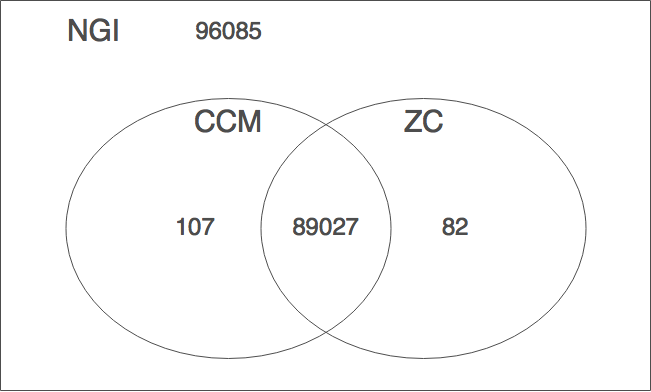
\includegraphics[width=0.6\linewidth]{figures/venn_geospatial_issues.png}
    \caption{Number of occurrences from the UB herbarium dataset classified within each geospatial issue class. \textit{NGI}: Records with no geospatial issues; \textit{CCM}: Country Coordinates Mismatch issue; \textit{ZC}: Zero Coordinates issue.}
    \label{fig:venn_geospatial_issues}
  \end{figure}

Records without geospatial issues comprise approximately $52\%$ of the dataset, and their coordinates are shown in Figure \ref{fig:occurrence_map}. Notice that the figure extent is constrained around the Brazilian territory, and records outside the canvas are omitted. Although most records deposited in the UB herbarium were collected in Brazil, there is also a considerable amount of records from many other countries (Figure \ref{fig:recs_by_cntry_state}a), that were been obtained from herbaria exchange activities or international recording expeditions. According to the herbarium description available from the \textit{Florescer project} webpage \footnotemark[\getrefnumber{footnote:florescer}], records from the Amazon and Atlantic forest were mostly exchanges under the curatorship of \textit{Dr. João Murça Pires} and \textit{Dr. Graziela Maciel Barroso}, respectively. A considerable part of international records were exchanges incorporated under the curatorship of \textit{Dr. George Eiten}.  


  \begin{figure}[!htb]
  	\centering
    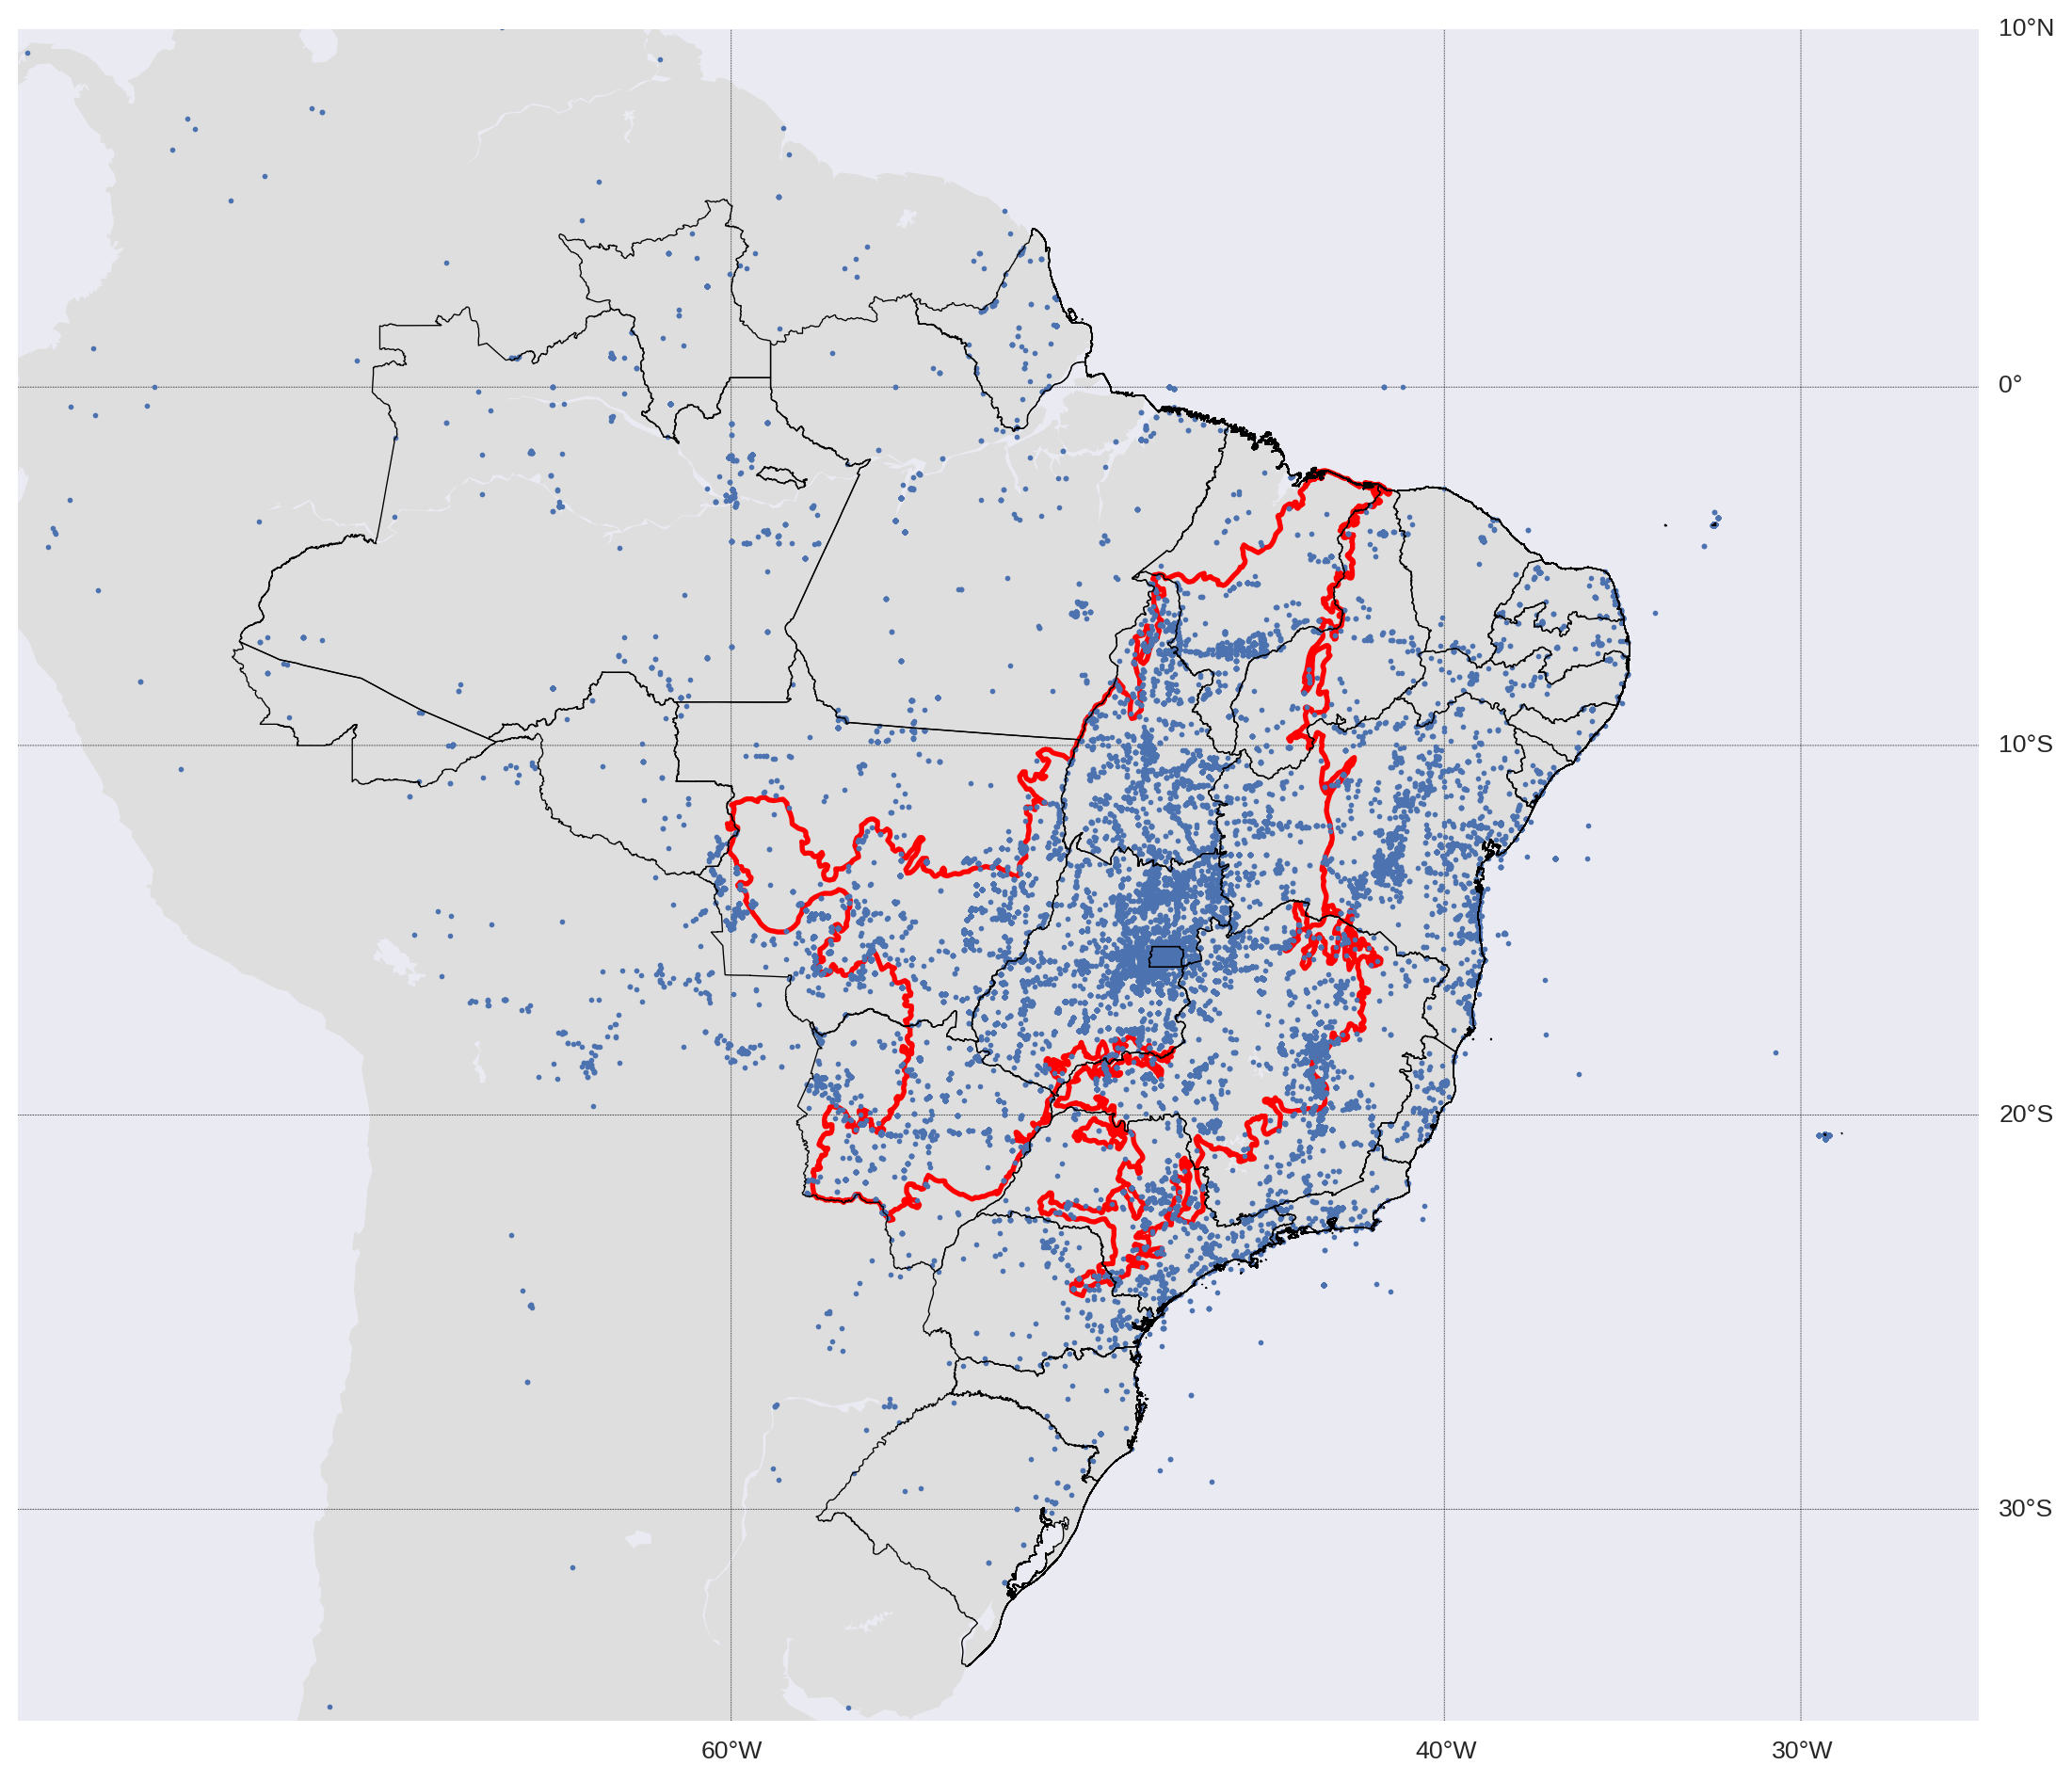
\includegraphics[width=\linewidth]{figures/occurrence_map.png}
    \caption{Geographic distribution of the occurrences from the UB Herbarium dataset near the Brazilian territory. Records without geospatial issues are placed in the map as blue dots. The area outlined in red represents the boundaries of the Cerrado biome.}
    \label{fig:occurrence_map}
  \end{figure}
  
  \begin{figure}[!htb]
  	\centering
    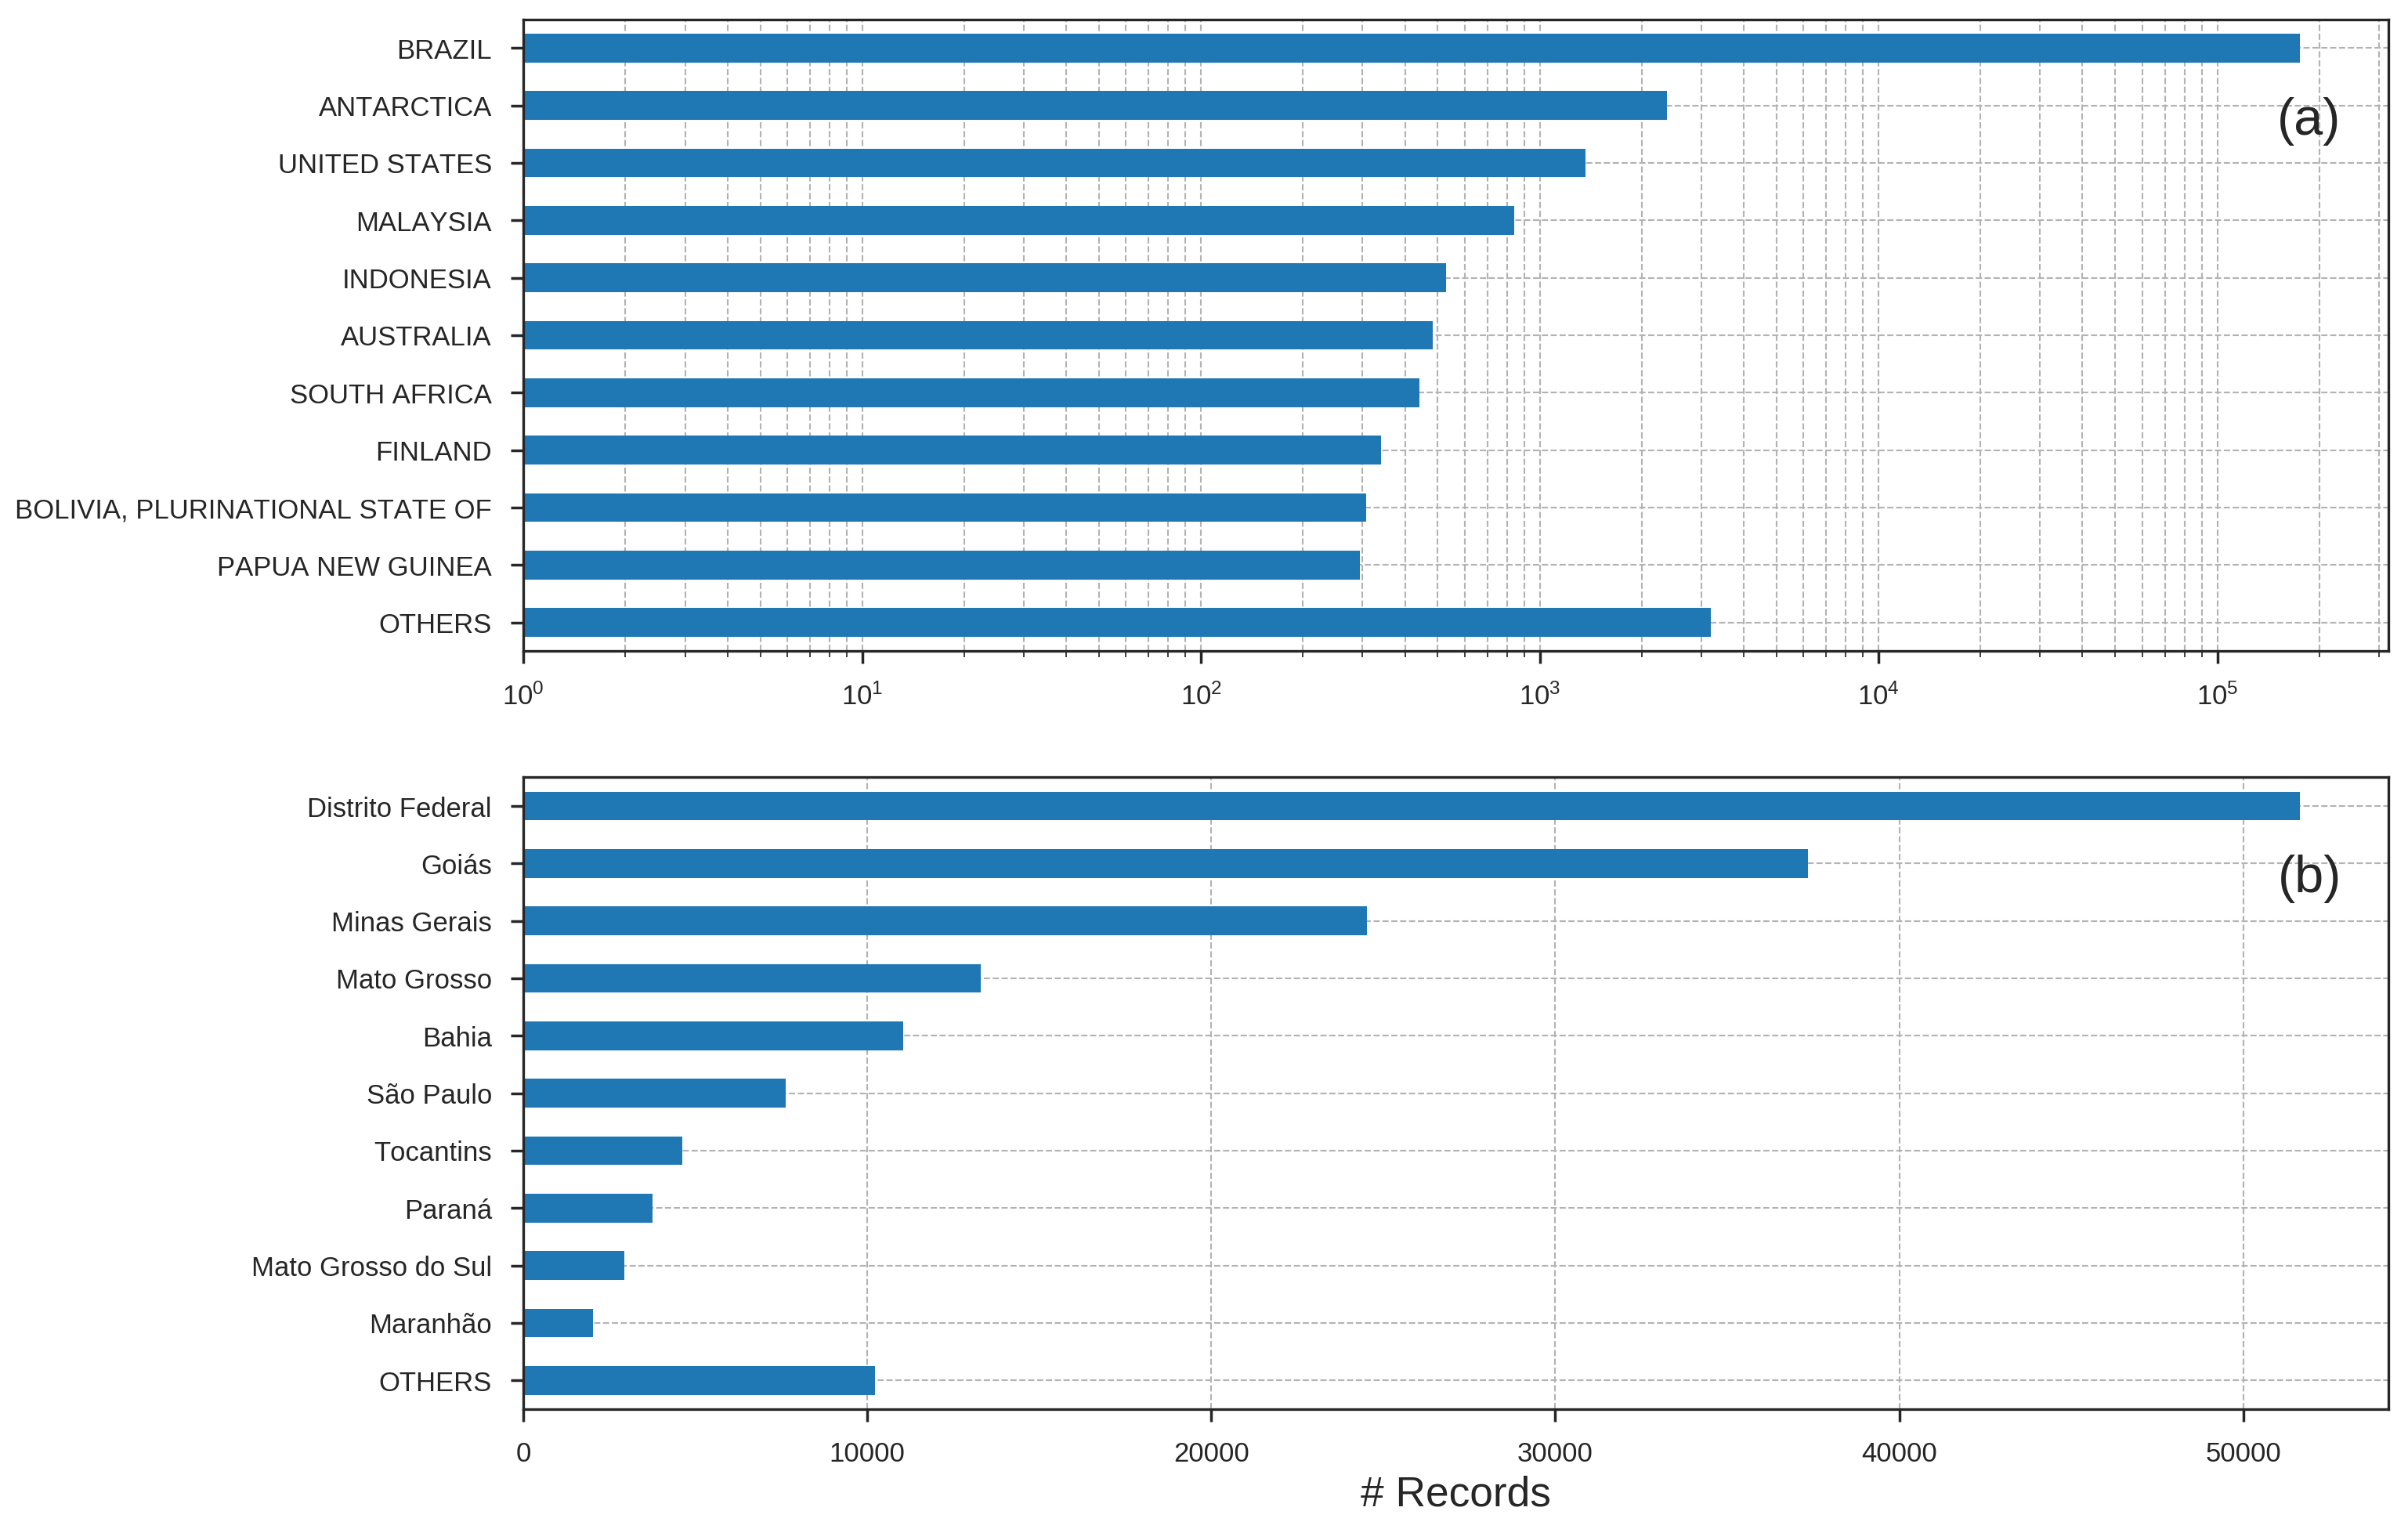
\includegraphics[width=\linewidth]{figures/recs_by_cntry_state.png}
    \caption{Top-10 countries (a) and top-10 Brazilian states (b) with most occurrence records deposited in the UB herbarium. Records from countries and states beyond the $10th$ position in the respective ranks are summed and assigned to \textit{OTHERS}.}
    \label{fig:recs_by_cntry_state}
  \end{figure}
  
Within the Brazilian territory, the Federal District was the most sampled federative unit despite its small area, followed by the state of Goiás (\ref{fig:recs_by_cntry_state}b). 
Such a geographic bias in the occurrences distribution can be explained by the fact that UB is physically located in the University of Brasilia, making it more viable for associated collectors to record in nearby locations.
Moreover, as UB is a national reference herbarium for species occurring the Cerrado biome, botanists working in Cerrado areas become more inclined to deposit their recordings in the institution.
In fact, figure \ref{fig:occurrence_map} shows that UB records are more densely concentrated within the Cerrado biome, mostly in the Central Brazil region. 


  
%%%%%%%%%%%%%%%%%%%%%%%%%%%%
%% Temporal characterization
% TODO: Include # species accumulation in the figure
Almost $98\%$ of the records contain information about their collection dates.
The oldest records in the herbarium dataset date from 1800.
However, more intensive collection activity started around 1960. Around 8000 records in the herbarium date up to that time (Figure \ref{fig:ub_records_timeseries}(c)). 
From 1950 to present, there are two apparent peaks in collection activity around year 1965 and 2013 (Figure \ref{fig:ub_records_timeseries}(a)). % Why?

  \begin{figure}[h!]
  	\centering
    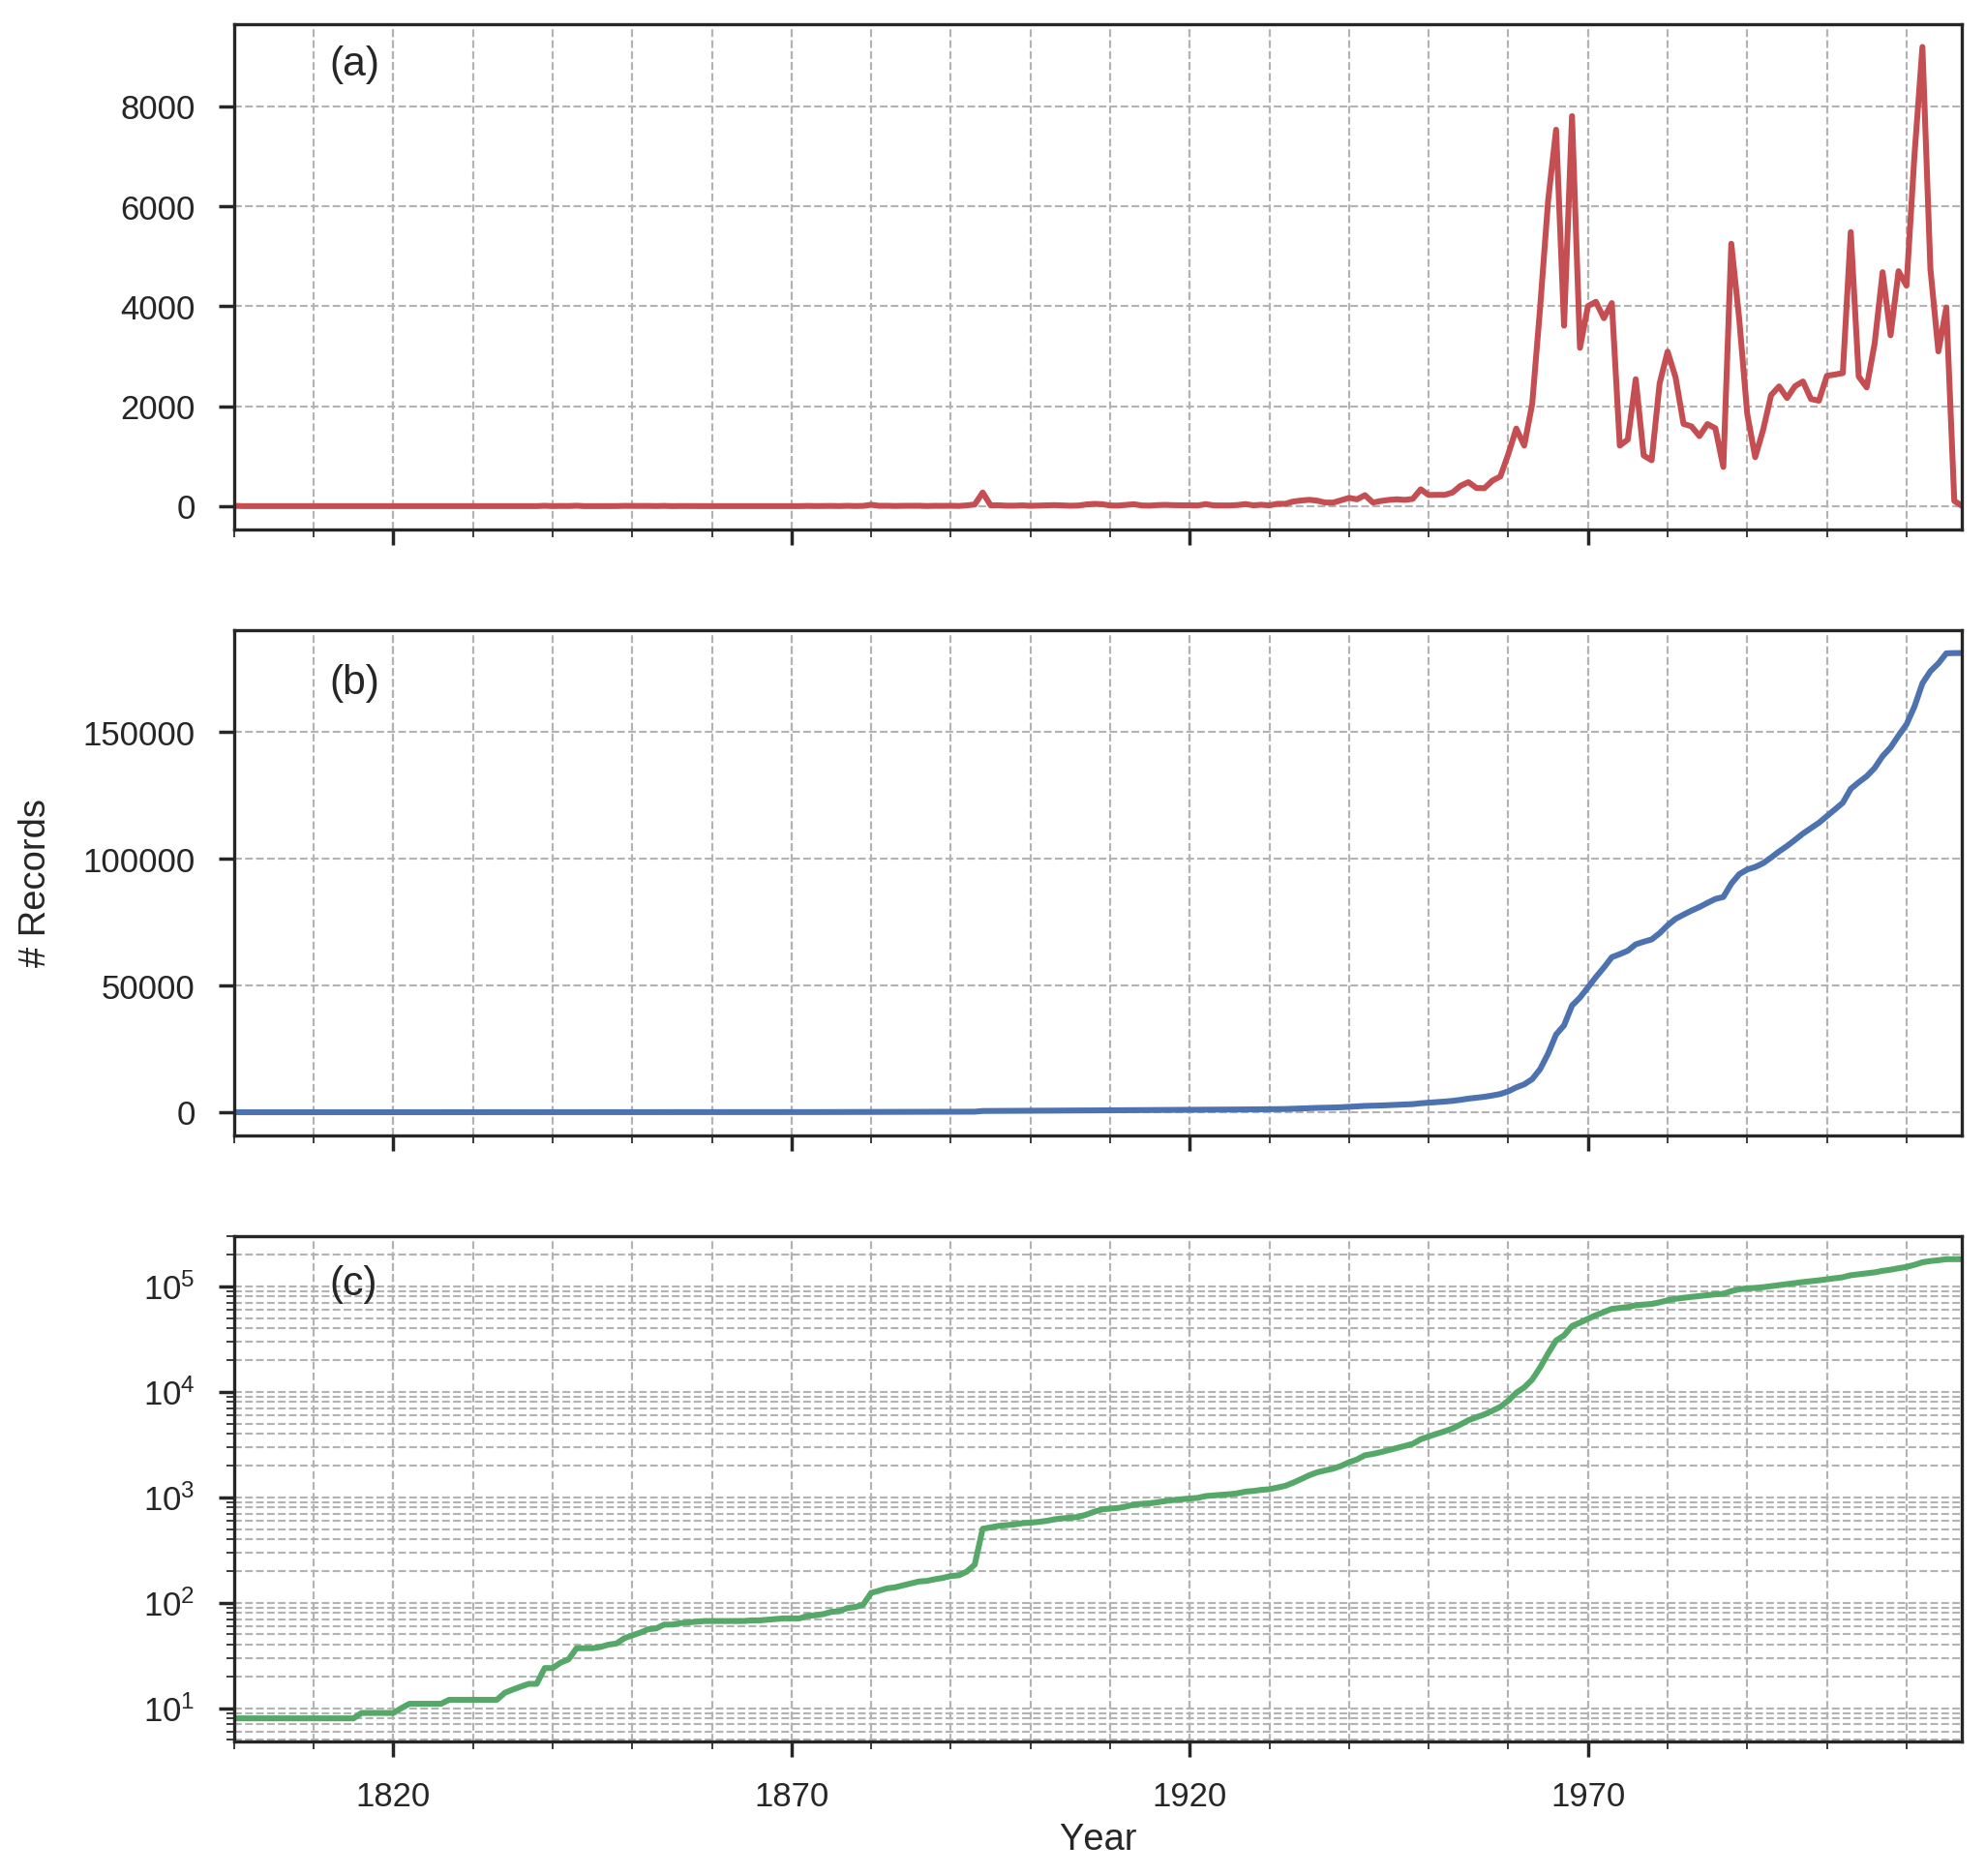
\includegraphics[width=\linewidth]{figures/ub_records_timeseries.png}
    \caption{Recording activities registered in the UB herbarium since 1800, aggregated by year. (a) Absolute record counts for each year. (b) Cumulative counts of records in a linear scale. (c) Cumulative counts of records using a logarithmic scale.}
    \label{fig:ub_records_timeseries}
  \end{figure}


%%%%%%%%%%%%%%%%%%%%%%%%%%%%%%
%%%%%%%%%%%%%%%%%%%%%%%%%%%%%%
%% Network models construction
\section{Network models construction}


% Build SCN
% What is the species with more collectors? What is the collector with more species?
% Average collector/species & species/collector  (with percentages)

For exploring the recording behavior of UB collectors in terms of their taxonomic preferences and collaborations we built a Species-collectors network model (SCN), linking collectors to the species they've recorded; and a Collectors coworking network (CWN), linking collectors who collaborated during field recording.

Some data preprocessing routines including names atomization and null values filtering were executed in the tabular dataset before it could be used to build the models. 
For the SCN we filtered out records with taxonomic resolution lower than species.
For the CWN model we only filtered out records with null entries for the collectors field.
Additionally, a previously elaborated names map for the UB dataset collectors was passed in during SCN construction, facilitating the process of remapping names variants to entities. 
Finally, nodes derived from noise entities such as \textit{``et. al"}, \textit{``Incógnito"}, \textit{``Ignorado"}, \textit{``Ilegível"} and \textit{``?"} were excluded from the network model right after its creation.




% ==========================
% Species-collectors Network
% --------------------------
\subsection{The UB Species-collectors Network}

The resulting network had a total of $6768$ collectors and $15344$ species nodes, with a total of $142647$ undirected edges connecting nodes from opposite sets. 
Average degree for the collectors and species set are respectively $21.08$ and $9.30$.

\paragraph*{Connected components.}
The UB SCN network is composed by a total of $351$ connected components, the largest of which (the giant component, or $c_1$) contains most nodes in the network ($93.6\%$ of the collectors and $95.0\%$ of the species). 
From a collector's perspective, the requirement for it to belong to the giant component is that it must have collected at least one species in common with another collector who is already included in the giant component. The same reasoning applies to species nodes as well by observing the inverse relationship.
Apart from the giant component, most other connected components contain as few as two or three nodes. These represent collectors who have never recorded a species in common with any collector from $c_1$; and conversely, species that have never been collected by any of those $c_1$ collectors.
One of those $350$ remaining connected components, however, is considerably larger than the others, with a total of $3$ collectors and $141$ species. We refer to it as the second largest component ($c_2$) throughout this section.

From all the records that form the giant component, $95.2\%$ are from Brazil, from which $53\%$ were recorded either in the Federal District or in the state of Goiás. 
Also, $c_1$ is mostly composed of species within phylum \textit{Tracheophyta} ($88\%$ of all records), followed by phylum \textit{Bryophyta} (mosses), comprising $8\%$ of the records. 
Component $c_2$, on the other hand, is represented by algae (phyla \textit{Charophyta}, \textit{Chlorophyta}, comprising $91.6\%$ of all records), bacteria (phylum \textit{Cyanobacteria} ($4.3\%$)) and other microscopic eukariotic organisms (phyla \textit{Euglenozoa}, \textit{Myzozoa} ($4.1\%$)), which are taxonomically distinct from the vast majority of species in the herbarium.
In addition, all records composing $c_2$ were collected in the Federal District.
The remaining components ($c_3,c_4,..., c_{351}$) include a total of $431$ distinct collectors and $446$ distinct species, and result from records mostly from outside Brazil ($79\%$ of them).
The most representative country is the United States, holding $23.9\%$ of the records, followed by Brazil with $21\%$. 
Considering the records from within Brazil, only $7.8\%$ of them were collected in the Federal District. Most of them ($59.2\%$) are from the southeast region, among which the state of São Paulo comprises $52.5\%$.

We have hypothesized some possible explanations for the existence of so many small connected components in the UB herbarium SCN with such characteristics. First, they could be a consequence of specimen exchange, a practice that is widely adopted among herbaria for collaboratively diversifying and distributing their collections \cite{Groom2014}. Exchange materials are typically duplicated exsiccates collected in field that a sender institution dispatches to a receiver institution. The receiver institution then incorporates those materials to its scientific collection, and ocasionally sends back to the other institution some duplicate exsiccates of its own.
From the receiver herbarium viewpoint the inclusion of records from exchanges usually adds new species and collectors, for they are a sample reflecting the sender institution's purpose and the interests of people associated to it. If both the collectors and species from such records were previously inexistent in the receiver collection, no links to $c_1$ or to any other connected component that already exists are formed. These records thus get included into its SCN network as nodes and edges composing new small connected components. We should overstate, however, that including exchange records does not necessarily create new connected components. New species or collectors could be included in $c_1$ in case either the species or at least one of the collectors associated to the exchange record are already linked to it.

A second situation that could potentially lead to isolated components in the network is when there are groups of very specialized collectors sampling very specific and distinct groups of organisms. 
Cryptic organisms such as algae, fungi and mosses are examples of groups which tend to be overlooked by botanists who are not directly interested on them. 
If collectors who record such groups also show a very high specificity towards them, it gets more likely that they lack links to other species which are more commonly recorded by the rest of the collectors, thus forming structures that are detached from the giant component. 
In case these collectors regularly deposit their materials in the herbarium it would be natural to observe them composing connected components with a relatively large number of species.
The connected component $c_2$, for instance, includes \textit{Ana Lúcia Tostes Leite} (\textit{leite,alta}), one of the herbarium's most relevant continental algae collector as shown in Table \ref{table:ub_collectors_florescer}.
She holds a total of $2757$ records, from $87$ distinct species, all of them being charophytes, a division of green algae (Figure \ref{fig:ub_scn_agg_family_general}, within polygon $ii$).



\paragraph*{Number of species per collector.}
Collectors contributing to the UB herbarium have, in average, recorded and successfully deposited approximately $21.1$ distinct species in that collection during their careers (Table \ref{table:ub_scn_degrees}). This value is obtained by computing the average degree $\langle k_{col} \rangle$ from all nodes in $S_{col}$ set, and would be equivalent to the expected number of species for a randomly selected collector if the SCN were a random network \cite{Albert2002}.
However, by visually inspecting the degree distribution of collectors in Figure \ref{fig:ub_scn_degree_dist}(b and d) we realize that the vast majority of collectors have recorded very few species. In fact, around $86.7\%$ of the collectors have degrees below or equal $floor(\langle k_{col} \rangle)$, and around $79\%$ have recorded $10$ or fewer species.
On the other hand, there are also some few collectors who have recorded much more species than the average, as it is the case of \textit{Howard S. Irwin} (\textit{irwin,hs}), with a total of $4535$ records of distinct species; and \textit{Carolyn E. B. Proença} (\textit{proenca,ceb}), with $1888$ distinct species. Nodes that are very intensely connected in the network are called hubs.

\begin{table}[t]
\caption{ Degree centrality metrics for the UB SCN model. For each nodes set the total number of nodes, average degree $\langle k \rangle$, top-10 highest-degree nodes and their respective degree $k$, weighted degree $k_w$ and normalized degree $k^*$ are listed.}
\begin{center}
	\caption{Some degree metrics for the UB SCN model. For each nodes set the total number of nodes, average degree $\langle k \rangle$, top-10 highest-degree nodes and their respective degrees $k$ are listed. We define $k^*$ as the maximum possible degree of a nodes set, a metric that represents the degree of a hypothetical node which is connected to every single node from the complementary set. Therefore $k/k^*$ is the proportion of nodes from the complementary set a given node is linked to.}
  \begin{center}
  \begin{tabular}{l c c c c c}
    & num of nodes & $\langle k \rangle$ & top-10 & $k$ & $k/k^*$ \\
   \hline    collectors & 6768 & 21.08 &
   \begin{tabular}[t]{{@{}c@{}@{}}}irwin,hs\\heringer,ep\\anderson,wr\\proenca,ceb\\ratter,ja\\faria,jeq\\eiten,g\\souza,rr\\harley,rm\\santos,rrb\end{tabular} &
   \begin{tabular}[t]{{@{}c@{}@{}}}4535\\2586\\2156\\1888\\1803\\1681\\1586\\1549\\1514\\1502\end{tabular} &
   \begin{tabular}[t]{{@{}c@{}@{}}}0.30\\0.17\\0.14\\0.12\\0.12\\0.11\\0.10\\0.10\\0.10\\0.10\end{tabular} \\ \\
    species & 15344 & 9.30 &
   \begin{tabular}[t]{{@{}c@{}@{}}}\textit{Myrcia splendens}\\\textit{Myrcia guianensis}\\\textit{Eugenia punicifolia}\\\textit{Casearia sylvestris}\\\textit{Palicourea rigida}\\\textit{Myrcia tomentosa}\\\textit{Qualea parviflora}\\\textit{Solanum lycocarpum}\\\textit{Piper aduncum}\\\textit{Miconia albicans}\end{tabular} &
   \begin{tabular}[t]{{@{}c@{}@{}}}388\\335\\266\\258\\241\\239\\232\\228\\209\\201\end{tabular} &
   \begin{tabular}[t]{{@{}c@{}@{}}}0.06\\0.05\\0.04\\0.04\\0.04\\0.04\\0.03\\0.03\\0.03\\0.03\end{tabular} \\ 
  \hline
  \end{tabular}
  \end{center}
  \label{table:ub_scn_degrees}

\end{center}
\label{table:ub_scn_degrees}
\end{table}

  \begin{figure}[t]
  	\centering
    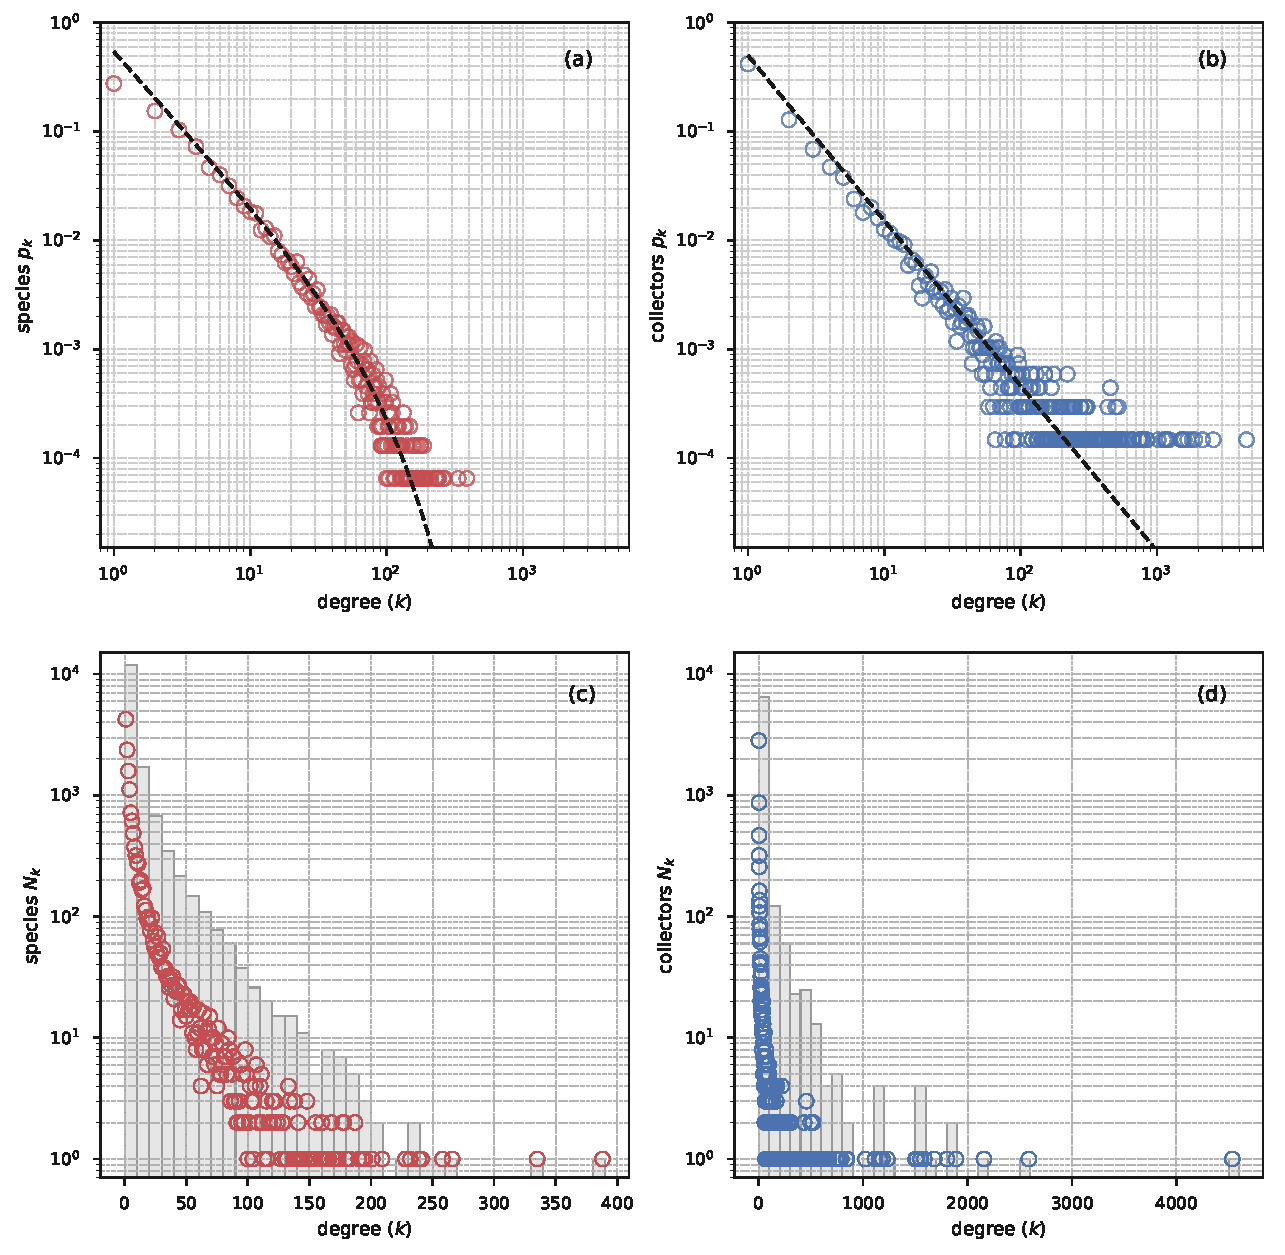
\includegraphics[width=\linewidth]{figures/casestudy_ub/scn_degree_dist}
    \caption{Degree distribution for both species ($a$ and $c$) and collectors ($b$ and $d$) nodes. The upper row plots show the probability $p_k$ of finding nodes with each degree value, using a log-log scale. The dashed curves represent power laws ($a$ has a tail cutoff) that best fit the SCN data, with $\alpha=1.38$ and $\alpha=1.52$ for plots $a$ and $b$, respectively. The exponential cutoff in $a$ is obtained by using $\lambda=0.014$. Plots in the lower row show the total number $N_k$ of nodes with each degree value, using a lin-log scale for enhancing interpretability. Histograms in the background group collectors using bin sizes $s=10$ and $s=100$ for plots $c$ and $d$, respectively.}
    \label{fig:ub_scn_degree_dist}
  \end{figure}

As opposed to random networks, in which extremely well connected nodes are unlikely to coexist with a large number of extremely poorly connected ones, the degree distribution observed for collectors in the UB SCN is better approximated by a power law $p(k) \sim k^{-\alpha}$, typically observed in many large real-world networks with the scale-free property \cite{Barabasi1999a}. 
The dashed line in figure \ref{fig:ub_scn_degree_dist}b is a power law fit for the $S_{sp}$ data, with $\alpha=1.52$. 
An apparently similar heavy-tailed distribution was recently reported by Barnabas Daru \textit{et. al} while investigating sampling bias in the digitized datasets of three distinct herbaria from Australia, South Africa and the United States \cite{Daru2017}.
They refer to the phenomenon in which a small subset of collectors is responsible for the majority of records as the \textbf{collector bias}.
  
Other useful degree centrality metrics shown in Table \ref{table:ub_scn_degrees} are the weighted degree $k_w$ and normalized degree $k^*$. The weighted degree for each collector node is computed by summing up weights assigned to each of the node's edges. Edges can be weighted according to any chosen attribute of its own, depending on the aspect of the connection the user wants to emphasize. Here we use the \textit{count} attribute, which holds the number of times the association between a collector and a species occurs. Formally, $k_w^{(u)} = \sum_{v} count(e_{u,v})$ for $v \in$ $neighbors(u)$. Differently from the degree, which gives the number of distinct species that have been recorded by a collector, the weighted degree of a collector can be interpreted as the total number of specimens (or occurrence records) collected by him/her. It is also worth to note that a node's $k_w$ is equivalent to the node's \textit{count} attribute, which is not to be confused to edges' homonymous attribute.

The intuition behind the normalized degree $k^*$ metric for a collector is to get the fraction of species from the entire $S_{sp}$ set it is connected to. More generally, we compare a node's degree to the maximum degree value that would be possible for nodes in the same set. In a bipartite model it turns out to be the node's degree divided by the size of the opposite set. Therefore, $k^{*(i)} = \frac{k^{(i)}}{|S_{sp}|}$, for each node $i \in S_{col}$. 
As stated by Borgatti \cite{Borgatti2015}, the advantage of using this normalized metric over the non-normalized degree $k$ is that it allows us to numerically compare centrality scores across nodes sets independently of their respective sizes. 
In our case data shows that collectors hubs tend to be more central than species hubs. The top collector \textit{irwin,hs} is linked to $30\%$ of the total diversity of the herbarium species, whilst the top species \textit{Myrcia splendens} has been recorded by $6\%$ of the herbarium collectors (Table \ref{table:ub_scn_degrees}). 



\paragraph*{Number of collectors per species.}
For the species nodes set ($S_{sp}$), the average degree $\langle k_{sp}\rangle \approx 9.5$, which can be interpreted as that species in the UB herbarium have been collected by approximately $9.5$ distinct collectors, in average. 
The total number of times each species has been recorded and the percentage of collectors that have recorded them at least once are given by the $k_w$ and $k^*$ metrics, respectively (Table \ref{table:ub_scn_degrees}).

The degree distribution for species nodes (Figure \ref{fig:ub_scn_degree_dist}(a and c)) shows a similar pattern to the distribution for collectors nodes, where a majority of very low degree nodes coexisting with a few hubs.
Most species (around $76.7\%$) hold degree values below or equal $floor(\langle k_{sp}\rangle)$, meaning they've been recorded by $9$ distinct collectors or less.
Yet, there are also some species that have been recorded by many more collectors than the average, as it is the case of \textit{Myrcia splendens} and \textit{Eugenia punicifolia}. Those top-10 species (Table \ref{table:ub_scn_degrees}) are in fact reasonably well-known, common and easily detectable species. Typical from cerrado physiognomies, \textit{Solanum lycocarpum} (\textit{lobeira}), \textit{Palicourea rigida} (\textit{chapéu-de-couro}), \textit{Qualea parviflora} (\textit{pau-terra}) are examples of species that are both very conspicuous and easy to identify.

A particularity that can be observed in the species degree distribution is the existence of a sharp tail decrease in the probability curve towards the highest degree nodes (Figure \ref{fig:ub_scn_degree_dist}a). Such behavior typically arises when the formation of a very high number of links is constrained by some system-specific factor \cite{Newman}.
% What is a possible explanation in this case? 
This behavior can be better adjusted by using a slight variant of the power law function $p(k) \sim e^{-\lambda k} k^{-\alpha}$, which is obtained by simply including an exponential cutoff term. We call this variant a truncated power law function. The dashed curve in Figure \ref{fig:ub_scn_degree_dist}a represents a truncated power with parameters $\alpha=1.38$ and $\lambda =0.014$, which was fit to the species degree distribution data.


\paragraph*{How densely connected are species and collectors?}
The density of the network is the ratio between the number of actual number of edges in the network and the maximum possible number of edges, in case every collector were linked to every species. This metric informs us how far the network is of being complete, in which case its density becomes $d=1$. For a bipartite network, density can be computed as $d = \frac{|E|}{|S_{col}| |S_{sp}|}$, where $|E|$ is the number of edges in the network and $|S_{col}|$ and $|S_{sp}|$ are the number of collectors and species, respectively.

The observed density for the overall UB species-collectors network is approximately $1.37 \times 10^{-3}$, meaning that the probability that we find an edge linking two arbitrary nodes from opposite sets is about $0.14\%$. Additionally, as shown in Figure \ref{fig:ub_scn_tax_agg_curves}, network density increases as we perform taxonomic aggregations onto successively higher-hierarchy ranks.

In most social networks, however, not all regions are equally dense, as entities usually do not connect to others randomly. Instead, entities with similar attributes or interests are more likely to establish new ties with each other than with dissimilar ones, leading to the formation of communities in the network.
% find parameters for network density (compare with other networks in literature)


\paragraph*{Communities of common interests.}
Communities in a species-collectors network are composed by groups of collectors who are specifically interested in a particular subset of organisms which are, in turn, not usually recorded by the rest of the herbarium collectors. 
As the number of edges linking members within a community is far greater than those connecting members to non-members, communities can be visually detected as clusters of nodes which are relatively well separated from the rest of the network when using force-directed algorithms \cite{Jacomy2014} for graph layout.

For a visual inspection of the community structure in the UB SCN we summarized it in basically two steps.
First we aggregated the SCN onto the \textit{family} rank following the routine described in section \ref{section:taxonomic_aggregation}, as it would be impractical to draw relevant conclusions from the network if every single species were plotted in the figure.
By performing the taxonomic aggregation, we reduced the number of $S_{sp}$ nodes (taxa) from $15344$ to $474$, although the number of edges (from $142647$ to $43803$) did not decrease in the same proportion (Figure \ref{fig:ub_scn_tax_agg_curves}).
This incurred in a $10 \times$ increase in network density, from $1.37\times 10^{-3}$ to $1.36\times 10^{-2}$.
In the second step of the summarization routine we removed collectors-families ties which occurred less than $20$ times throughout the entire dataset by filtering edges based on their \textit{count} attribute.
As this edges filtering routine resulted in many isolated collectors, most of which novice collectors with low absolute recording counts, we also omitted them for improving figure readability.

\begin{figure}[!ht]
  	\centering
    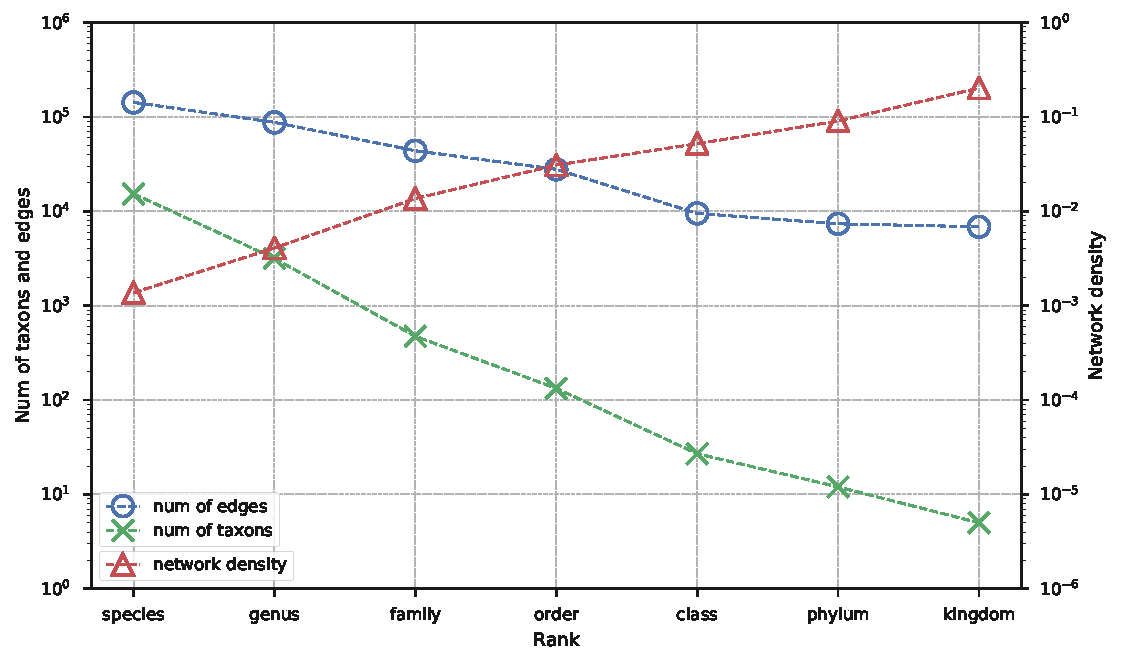
\includegraphics[width=\linewidth]{figures/casestudy_ub/scn_tax_agg_curves.pdf}
    \caption{ Number of taxa ($S_{sp}$ nodes), edges and network density for UB SCN aggregations onto successive taxonomic ranks. }
    \label{fig:ub_scn_tax_agg_curves}
  \end{figure}

\afterpage{
  \begin{figure}[!ht]
  	\centering
    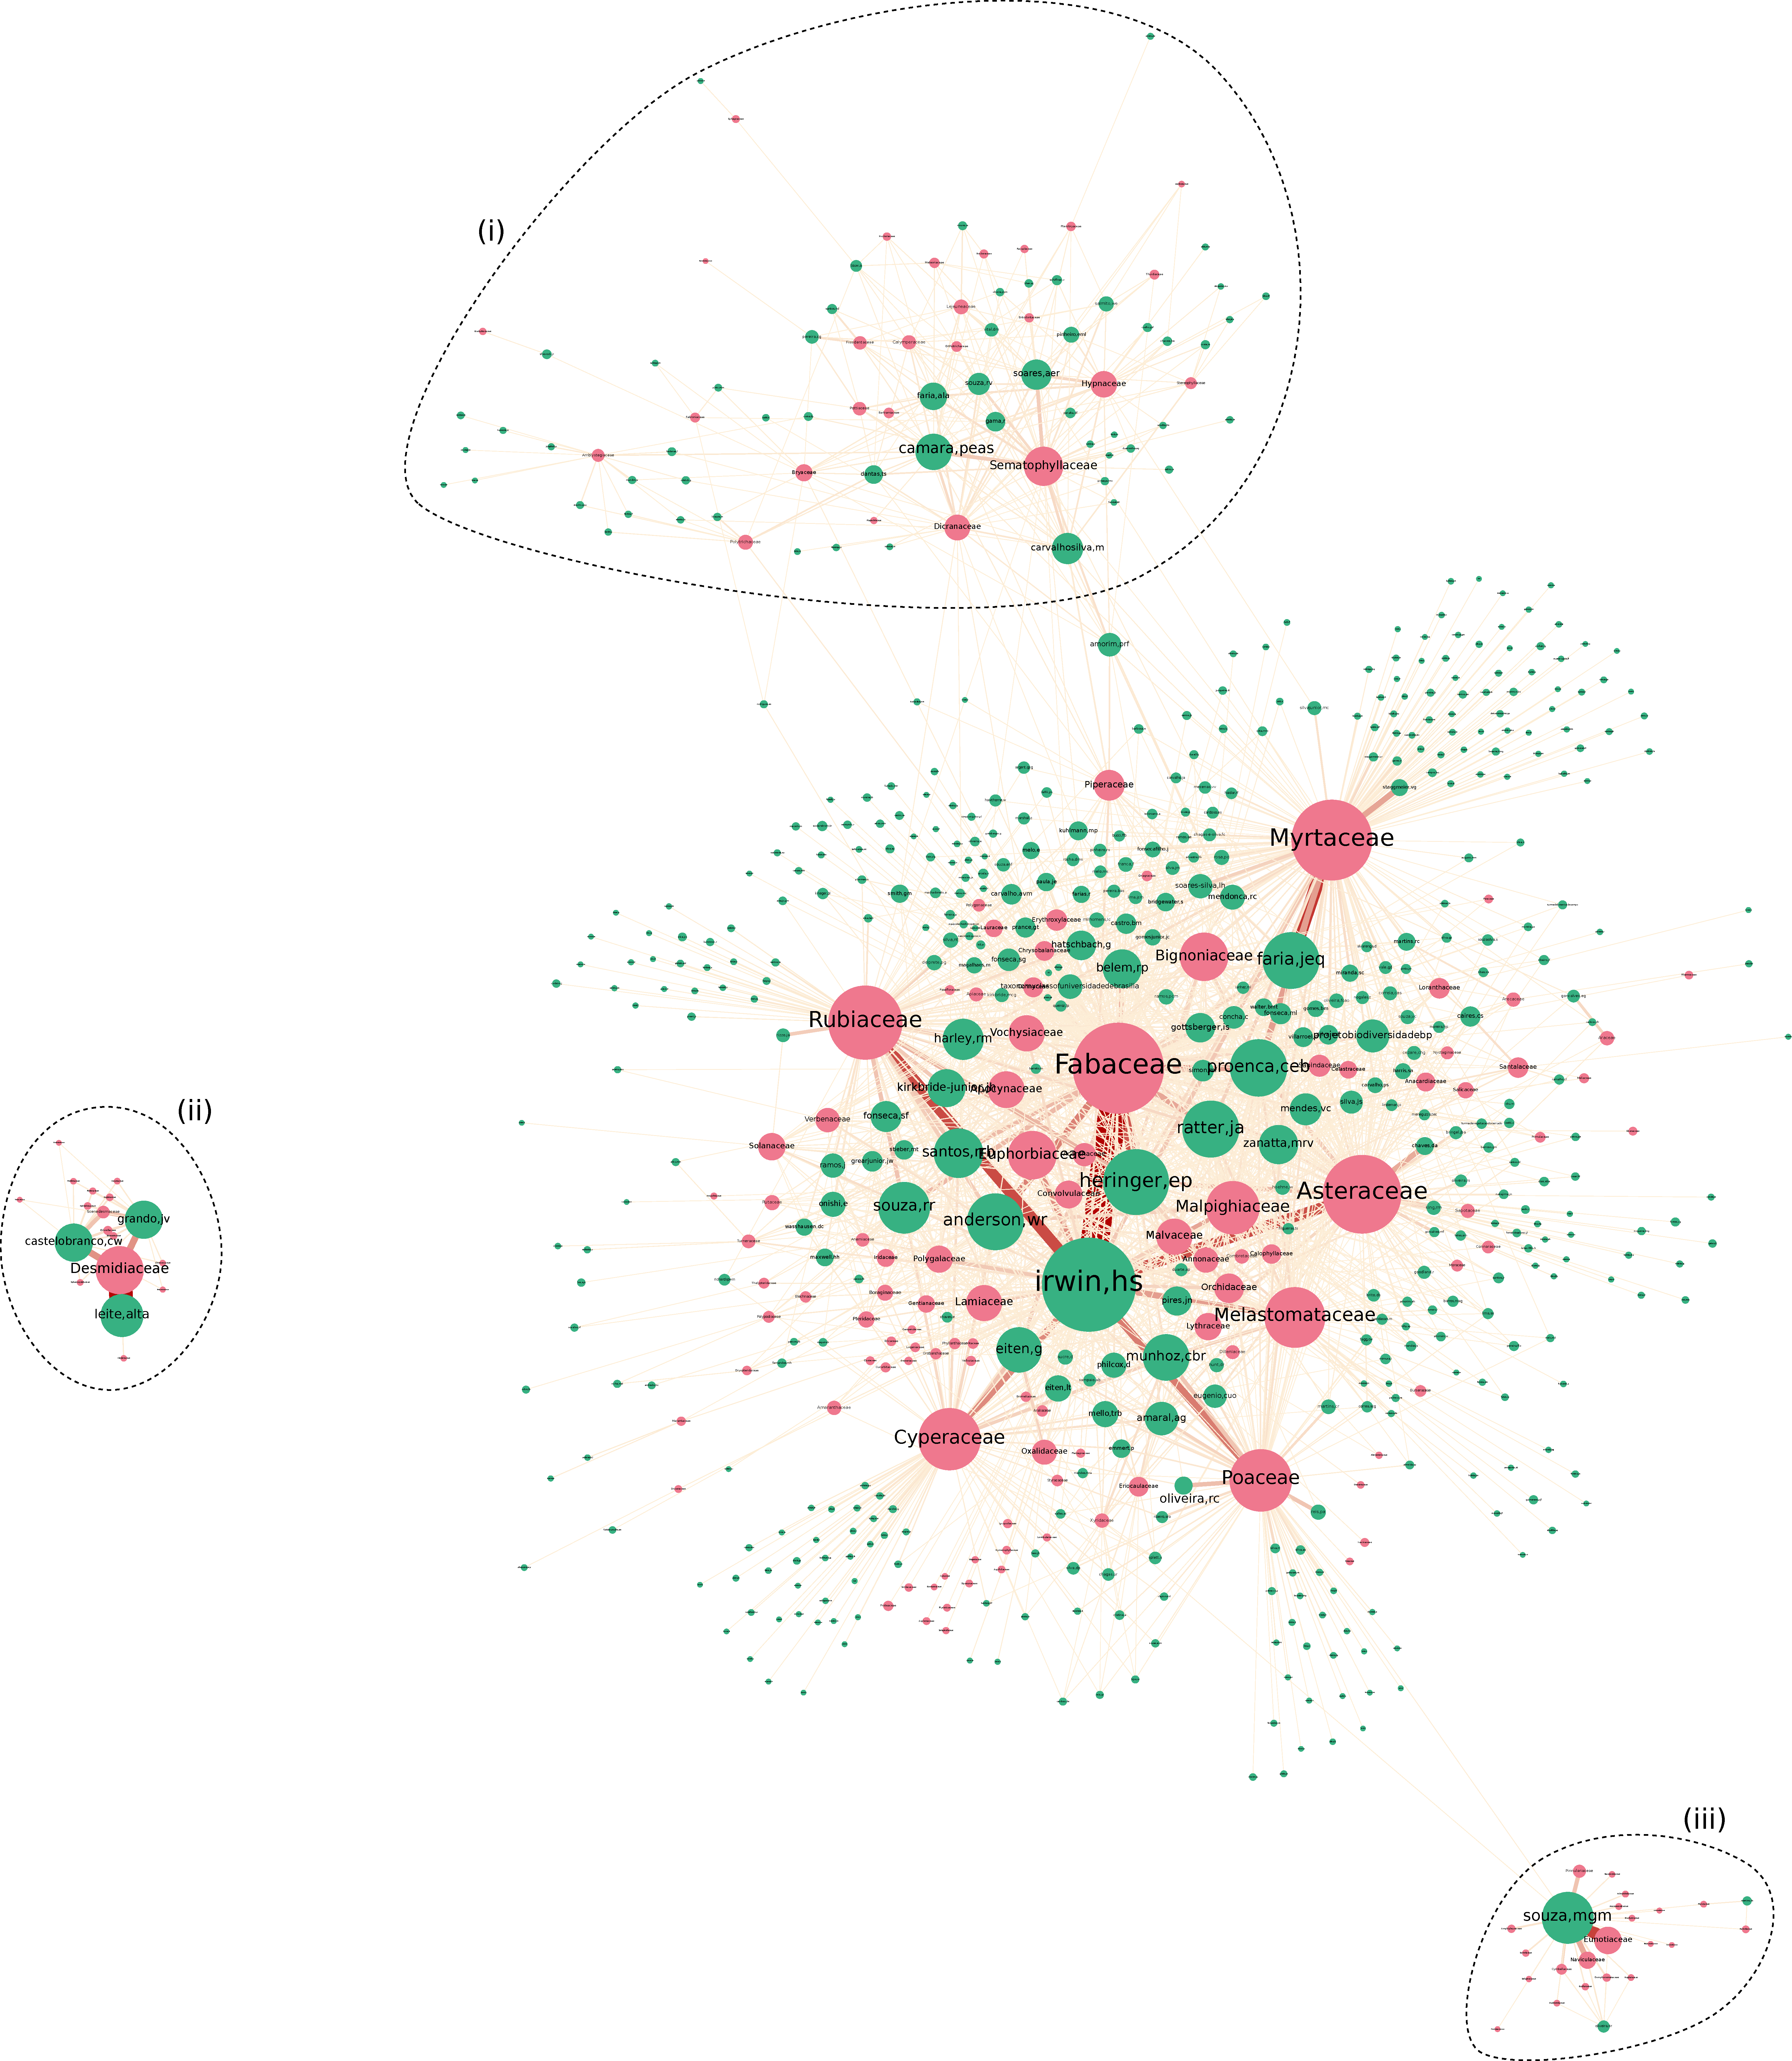
\includegraphics[width=\linewidth]{figures/casestudy_ub/scn_agg_family_general.pdf}
    \caption[alt]{ General aspect of the UB SCN network taxonomically aggregated onto the family rank. Species and collectors are respectively represented as pink and green nodes, and edges are weighted according to their \textit{count} attribute. Nodes sizing is based on their \textit{count} attribute, whilst edges color and width reflect their weight. For improving visualization we first filtered out edges with weight lower than $20$ and then omitted isolated nodes from the resulting graph. Nodes within poligons $(i)$, $(ii)$ and $(iii)$ compose visually distinguishable communities. Graph layout was computed using the \textit{ForceAtlas2} algorithm \cite{Jacomy2014}. For a better visualization experience refer to the interactive graph in the author's personal web page\footnotemark. }
    \label{fig:ub_scn_agg_family_general}
  \end{figure}
  \footnotetext{ \url{https://pedrosiracusa.github.io/networks/ub_scn_agg_family} }
}

Three communities are visually distinguishable from the central region of the network, which we'll refer to as the network core (Figure \ref{fig:ub_scn_agg_family_general}).
Although the network core could be considered a community \textit{per se}, we prefer to think of it as a region of the network that best reflects the overall interests of the majority of the most productive collectors composing the herbarium.
Nevertheless, collectors from the network core still vary considerably regarding their recording interests, as can be verified by inspecting the sets of taxa they're linked to as well as the strength of each connection. 
Those who have sampled organisms from many distinct families (and are thus considered to display a generalist collecting behavior) are placed more centrally in the network core by the layout algorithm, whereas specialists are consequently pushed towards the borders of the network core, as nearer as possible to their most recorded taxa.

\textit{Howard S. Irwin} (\textit{irwin,hs}) is the collector with most records in the network, having intensively sampled organisms from many distinct families, especially from the most central ones (illustrated in Figure \ref{fig:ub_scn_agg_family_general} as the biggest pink nodes).
The majority of his records are, in descending order, from families \textit{Fabaceae}, \textit{Rubiaceae}, \textit{Asteraceae}, \textit{Poaceae} and \textit{Cyperaceae}. 
He is also the collector holding the highest number of records for those families.
An interesting fact is that although \textit{Myrtaceae} is the second most recorded family in the UB dataset (with a total of $10951$ records), it was relatively overlooked by \textit{irwin,hs}, having himself contributed with only $399$ \textit{Myrtaceae} records. 
Instead, the main \textit{Myrtaceae} collector in the herbarium is \textit{Jair E. Faria} (\textit{faria,jeq}), who apparently has a preference towards this family, as it composes approximately $31.0\%$ of his entire records set. 
It could be insightful to investigate why a generalist collectors such as \textit{Irwin}, who mostly contributed to the herbarium in the context of the Central Brazil expedition (see Table \ref{table:ub_collectors_florescer}), was not very interested in such a predominant family from the Cerrado biome as \textit{Myrtaceae} (Figure \ref{fig:ub_scn_agg_family_general} ).
\textit{Carolyn E. B. Proença} (\textit{proenca,ceb}) is another key collector of this family, although she also seems interested, to the same extent, in families \textit{Fabaceae} and \textit{Asteraceae}. 
Moreover, the figure also makes it easy to detect collectors who exclusively (or almost exclusivelly) collect each family, as it is the case of \textit{Vanessa G. Staggmeier} (\textit{staggmeier,vg}) for \textit{Myrtaceae} and \textit{Regina C. Oliveira} (\textit{oliveira,rc}) for \textit{Poaceae}.

Community $i$ represents a large part of the \textit{Cryptogams Lab}\footnote{\url{http://labcriptounb.blogspot.com.br/}} collectors team, together with the taxa they're most interested in. 
The lab is part of the University of Brasília department of botany, having \textit{Paulo Eduardo A. S. Câmara} (\textit{camara,peas}), \textit{Micheline Carvalho Silva} (\textit{carvalhosilva,m}) and \textit{Maria das Graças M. de Souza} (\textit{souza,mgm}) as the principal investigators. 
%
The first two researchers, which have been included in community $i$, are mostly interested in bryophytes (mosses and liverworts), mainly those from families \textit{Sematophyllaceae}, \textit{Hypnaceae} and \textit{Dicranaceae}.
\textit{Micheline C. Silva}, however, also shows interest towards \textit{Piperaceae}, a family of flowering plants that has also been considerably recorded by collectors from the network core. 
Therefore, \textit{Piperaceae} is an important node connecting community $i$ to the network core, as it intermediates many paths between collectors from both network regions.
%
Some PhD and MSc students from the cryptogams lab including \textit{Abel Eustáquio R. Soares} (\textit{soares,aer}), \textit{Allan Laid Alkimim Faria} (\textit{faria,ala}), \textit{Ronaldo Viveiros de Sousa} (\textit{souza,rv}), \textit{Tamara Silva Dantas} (\textit{dantas,ts}), \textit{Renato Gama} (\textit{gama,r}) and \textit{Eliana Marília Lima Pinheiro} (\textit{pinheiro,eml}) have also been placed in community $i$, and their closeness to their academic supervisor \textit{`camara,peas'} reflect their common taxonomic interests in bryophytes.

Although she is one of the principal investigators of the \textit{Cryptogams Lab}, \textit{`souza,mgm'} was placed in community $iii$ instead of $i$ due to her taxonomic interest towards algae, a taxonomic group which is overlooked by the vast majority of collectors in the herbarium, including bryophytes collectors. 
She is mostly interested in families \textit{Eunotiaceae}, \textit{Naviculaceae}, \textit{Pinnulariaceae}, which compose a group of algae known as diatoms.
There are two more collectors in community $iii$.
Together with \textit{`souza,mgm'}, \textit{Roni Ivan Rocha de Oliveira} (\textit{oliveira,rir}) was a member of a survey on the diatoms acquatic biota of the Paranã River, during years 2002 and 2003.
\textit{Drielle dos Santos Martins} (\textit{martins,ds}) was an undergraduate student and a lichen collector, having been supervised by \textit{souza,mgm}.

Another community of algae collectors is the one formed by \textit{Ana Lúcia Tostes de Aquino Leite} (\textit{leite,alta}), \textit{João Vademar Grando} \textit{grando,jv} and \textit{Christina Wyss Castelo Branco} (\textit{castelobranco,cw}) (community $ii$), which also happens to be the connected component $c_2$ itself.
\textit{Ana Lúcia Leite} has intensely collected continental green algae from family \textit{Desmidiaceae} in the Federal District while pursuing her MSc degree at the University of Brasília.
During that period she has also collected some specimens from another green algae family, \textit{Closteriaceae}, which has not been recorded by anyone else from the UB herbarium.
She is regarded as one of the UB historically relevant collectors (Table \ref{table:ub_collectors_florescer}).
%
\textit{João Grando} and \textit{Christina Castelo Branco} were also MSc students at the University of Brasília, both working under the academic supervision of Dr. \textit{Antônio José de Andrade Rocha} (not included in the UB dataset).
Besides green algae (families \textit{Desmidiaceae}, \textit{Scenedesmaceae}, \textit{Chlorellaceae} \textit{Selenastraceae} \textit{Hydrodictyaceae}), they have also collected other types of microscopic organisms, such as euglenophytes (family \textit{Euglenaceae}) and cyanobacteria (families \textit{Nostocaceae}, \textit{Oscillatoriaceae}, \textit{Chroococcaceae} and \textit{Pseudanabaenaceae}). 
All those organisms are typical of limnic systems.
 

We could use a whole set of modularity detection algorithms in order to further split the network core and identify communities which are visually less conspicuous. 
However, if we used general modularity algorithms --- appropriate for one-mode graphs --- for analyzing non-projected bipartite networks, a set of bipartite constraints and assumptions would be systematically ignored \cite{Borgatti2015}.
A common practice among the statistical physics community for detecting communities in bipartite networks has been to first obtain bipartite projections and then running unipartite community detection algorithms for each of them, separately.
In order to minmize information loss, obtaining weighted bipartite projections is preferred over unweighted, as the latter have shown to produce poor results \cite{Guimera2007}.

In order to investigate more thoroughly communities of common interests under complementary perspectives we projected the family-aggregated SCN network shown in Figure \ref{fig:ub_scn_agg_family_general} into both the collectors (Figure \ref{fig:ub_scn_family_projCol_communities}) and the species sets (Figure \ref{fig:ub_scn_family_projSp_communities}), using the approach described in section \ref{section:scn_projection}.
We used the species bag / quorum similarity rule (expression \ref{equation:cosine_similarity}) for weighting the edges in the resulting unipartite networks.


% ======================
% The Col set projection
% TODO
%   - explain that nodes sizing in the figure represent the number of records for each collector in the herbarium dataset
\paragraph*{Communities in the collectors projection.}
\begin{figure}[!ht]
  	\centering
    \includegraphics[width=\linewidth]{figures/casestudy_ub/scn_family_projCol_communities.pdf}
    \caption{ Communities in the collectors-projection of the family-aggregated SCN in figure \ref{fig:ub_scn_agg_family_general}, in which edges with weights lower than $20$ were removed as well as isolated nodes. In order to improve visualization, communities with scores lower than $500$ were also omitted from the figure. Colors are used to distinguish communities.}
    \label{fig:ub_scn_family_projCol_communities}
\end{figure}
The collectors projection of the family-aggregated UB SCN network has a total of $6768$ nodes and $5,431,799$ edges, with average node degree $\langle k \rangle = 1605$.
Although the taxonomic aggregation process does not change the number of nodes at all in a collectors projection of a SCN, the number of edges connecting collectors together increases signifficantly from lower-rank towards higher-rank aggregations, which means they also become denser.
In fact, the density of our family-aggregated SCN collectors projection is $2.37 \times 10^{-1}$, while the same projection at the species resolution is almost $10$ times sparser, with a density of $3.64 \times 10^{-2}$. 
This happens because higher-level taxa represent broader ranges of organisms, and thus assume ties from all lower-rank taxa they are composed of.
In other words the lowest the taxonomic resolution of the network model is, the most inclusive are taxa modeled as nodes, making it more likely that collectors record at least one specimen belonging to it. 

% Similarity between collectors TODO
Another issue is that collectors with very few records in the dataset are more likely to have recorded identical sets of taxa by chance, leading to identical species bags.
As a consequence they are tied by edges with similarity very close to $1$.
This explains the formation of many fully connected regions containing low-degree nodes, which contribute to increasing network density.
More experienced collectors can be observed to have high similarity with others, but it is unlikely to be very close to $1$.
%% PLOT max similarity vs degree

We could reduce the density of the projected network by both ignoring nodes with very low degrees and ignoring weaker ties, which form between collectors who are less similar in their species bags.
For that we define a filtering routine, which consists of iterating through all entries $A_{i,j}$ of the network's biadjacency matrix and setting them to $0$ in case their respective values fall below a user-defined filter threshold $\phi$.
Acceptable values for the filtering coefficient $\phi$ range within the interval $[0,1[$, and represents the minimum similarity score that should be observed for a pair of collectors for their tie to be considered relevant.
Figure \ref{fig:ub_scn_filter_thresh}(a) illustrates the effect of increasing $\phi$ on the density of the UB SCN collectors projection, under three distinct taxonomic resolutions.
Although the three curves show a similar behavior, aggregations at lower taxonomic ranks show more pronounced drops, especially in the region where $\phi$ ranges from $0$ to $0.6$.
In addition, we verify that higher-rank aggregations lead to denser networks for all possible values of $\phi$.

\begin{figure}[!ht]
  	\centering
    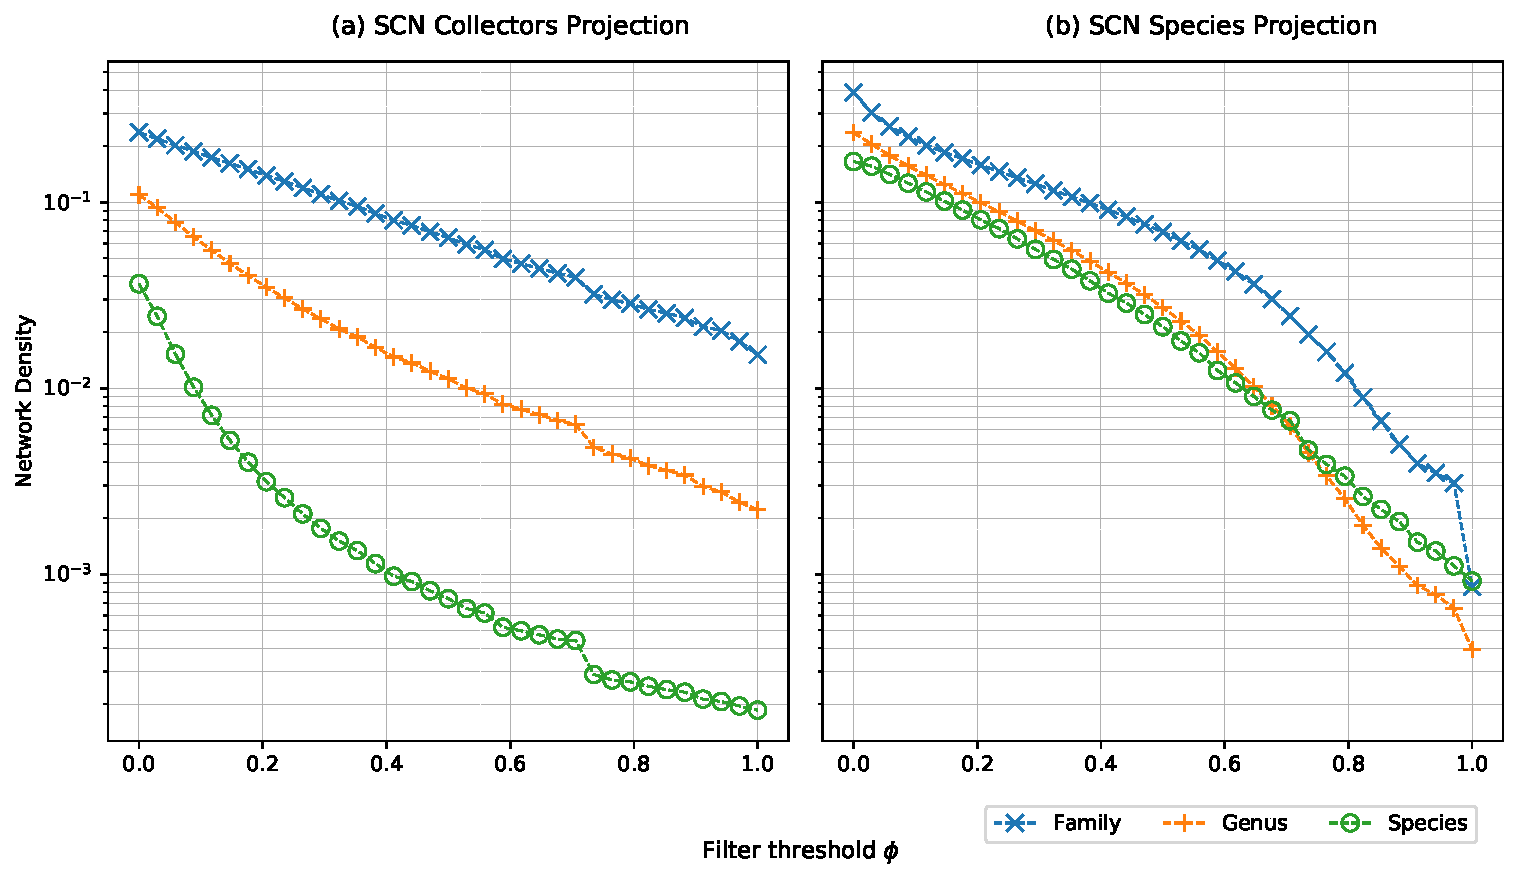
\includegraphics[width=\linewidth]{figures/casestudy_ub/scn_filter_thresh.pdf}
    \caption{ Reduction in the density of SCN collectors (a) and species (b) projections as a consequence of increasing filtering threshold $\phi$. Curves represent the SCN networks aggregated by family (blue), genus (orange) and at the original taxonomic resolution of species (green). }
    \label{fig:ub_scn_filter_thresh}
\end{figure}

In order to investigate the formation of communities in the collectors projection we first filtered collectors ties by setting $\phi = 0.8$.
This means only edges holding similarity scores equal or higher than $0.8$ were kept, while weaker ones were discarded.
This process led to the formation of many small connected components (or \textit{islands}), many of which composed of a single collector.
An additional step in the filtering process was thus required for removing less relevant connected components from the network.
In order to calculate the relevance of a component we defined a simple relevance score which adds up the the values associated to the \textit{count} attribute of each node composing it.
We then removed all islands with score lower than $500$.



% Communities
We applied the \textit{Louvain} heuristic method for community detection \cite{Blondel2008}, which maximizes modularity scores in the network in successive steps.   
The result is an optimized division of the network into modules within which nodes are more densely connected with each other than with external ones.
We also computed the overall taxa composition for each group by summing up the species bags of each of their collectors, which we show as percentages in Table \ref{table:ub_scn_family_projCol_composition}.


\begin{sidewaystable}
\begin{table}[H]
  \caption{Taxa composition for each community as illustrated in Figure \ref{fig:ub_scn_family_projCol_communities}. The total number of distinct taxa, together with the percentages of the top-3 most recorded ones in each community are given.}
  \begin{center}
  \begin{tabular}{r r l l l l}
      community & num of taxa & top taxon & 2nd taxon & 3rd taxon \\
      \hline
0 & 15 & Asteraceae (72.7\%) & Fabaceae (9.1\%) & Melastomataceae (5.2\%) \\
1 & 24 & Cyperaceae (50.4\%) & Fabaceae (9.9\%) & Oxalidaceae (7.2\%) \\
2 & 28 & Fabaceae (58.8\%) & Myrtaceae (8.6\%) & Rubiaceae (6.0\%) \\
3 & 27 & Poaceae (40.4\%) & Cyperaceae (12.5\%) & Asteraceae (7.5\%) \\
4 & 37 & Myrtaceae (62.0\%) & Fabaceae (7.7\%) & Asteraceae (4.3\%) \\
5 & 11 & Rubiaceae (82.7\%) & Myrtaceae (4.6\%) & Fabaceae (3.0\%) \\
6 & 104 & Fabaceae (18.8\%) & Rubiaceae (10.1\%) & Myrtaceae (8.4\%) \\
7 & 27 & Sematophyllaceae (26.8\%) & Hypnaceae (16.0\%) & Dicranaceae (13.8\%) \\
8 & 14 & Desmidiaceae (31.4\%) & Scenedesmaceae (18.9\%) & Chlorellaceae (9.7\%) \\
9 & 23 & Eunotiaceae (35.4\%) & Naviculaceae (15.2\%) & Pinnulariaceae (11.2\%) \\
10 & 2 & Desmidiaceae (97.5\%) & Closteriaceae (2.5\%) \\
11 & 18 & Poaceae (14.3\%) & Fabaceae (13.2\%) & Santalaceae (11.1\%) \\
12 & 4 & Amblystegiaceae (63.6\%) & Polytrichaceae (22.6\%) & Dicranaceae (10.4\%) \\
13 & 5 & Orchidaceae (73.6\%) & Myrtaceae (9.8\%) & Araceae (7.2\%) \\
14 & 9 & Santalaceae (34.5\%) & Loranthaceae (17.4\%) & Myrtaceae (13.4\%) \\
15 & 1 & Melastomataceae (100.0\%) \\
16 & 6 & Fissidentaceae (53.2\%) & Calymperaceae (17.3\%) & Pottiaceae (16.8\%) \\
17 & 7 & Rubiaceae (20.5\%) & Fabaceae (18.8\%) & Dicranaceae (16.2\%) \\
18 & 6 & Arecaceae (36.1\%) & Myrtaceae (25.4\%) & Fabaceae (15.4\%) \\
19 & 4 & Calophyllaceae (38.1\%) & Fabaceae (28.1\%) & Asteraceae (23.8\%) \\
      \hline
  \end{tabular}
  \label{table:ub_scn_family_projCol_composition}
  \end{center}
\end{table}
\end{sidewaystable}


The collectors projection has a total of $20$ communities, $7$ of which are included in a giant component (Figure \ref{fig:ub_scn_family_projSp_communities}), which does not overlap with the giant component in Figure \ref{fig:ub_scn_family_projCol_communities}.
The biggest community in the giant component is \textit{grp $6$}, including some of the most important UB collectors among which \textit{`irwin,hs'}, \textit{`heringer,ep'}, \textit{`anderson,wr'}, \textit{`ratter,ja'} and \textit{`proenca,ceb'}.
These are generalist collectors, having recorded $104$ from a total of $161$ distinct families, being families \textit{Fabaceae} ($18.8\%$ of the group interest), \textit{Rubiaceae} ($10.1\%$) and \textit{Myrtaceae} ($8.4\%$) the most recorded ones. 
%
The giant component also includes other smaller communities showing predominant interests towards families \textit{Myrtaceae} (\textit{grp} $4$), \textit{Fabaceae} (\textit{grp} $2$), \textit{Poaceae} (\textit{grp} $3$), \textit{Asteraceae} (\textit{grp} $0$), \textit{Cyperaceae} (\textit{grp} $1$) and \textit{Rubiaceae} (\textit{grp} $5$)

Apart from the giant component there are $7$ other connected components and $6$ isolated nodes, each of them making a distinct community.
The second biggest connected component (\textit{grp{$7$}}) includes a more generalist part of the bryophytes collectors within polygon $(i)$ in Figure \ref{fig:ub_scn_agg_family_general}, where the most recorded family is \textit{Sematophyllaceae} ($26.8\%$), followed by \textit{Hypnaceae} ($16.0\%$) and \textit{Dicranaceae} ($13.8\%$). 
Another part of the bryophytes collectors was split into a distinct community (\textit{grp $12$}), more specialized in family \textit{Amblystegiaceae} ($63.6\%$).

Algae collectors from polygon $(ii)$ (Figure \ref{fig:ub_scn_agg_family_general}) are also split in two distinct communities.
\textit{João Vademar Grando} and \textit{Christina Wyss Castelo Branco} are placed in \textit{grp 8} and \textit{Ana Lúcia Tostes Leite} is represented as an isolated node (\textit{grp $10$}).
\textit{Maria das Graças M. de Souza} (within polygon $(iii)$ in Figure \ref{fig:ub_scn_agg_family_general}) is also represented as an isolated node, composing a community of a single collector.
This happens because these collectors are signifficantly distinct from the rest of the herbarium in their recording behavior, such that no strong similarities are observed with any other collector.

Although Table \ref{table:ub_scn_family_projCol_composition} gives some intuition on the main taxonomic groups that compose the interests of each community, it is not very informative on how community-specific each of those families are.
Family \textit{Fabaceae}, for instance, has been relatively more recorded by collectors from community $2$ (with $58.8\%$ of the records in that community), although it is also included as a top-3 taxon in communities $0$, $1$, $4$, $5$, $6$, $11$, $17$, $18$ and $19$.
This makes it non-specific, in that collectors in many communities have demonstrated interests towards recording it.
In contrast, family \textit{Desmidiaceae} is more community-specific, as it is only recorded by algae collectors composing communities $8$ and $10$ (both comprising together only $3$ collectors).
Moreover, it is also relevant to identify groups of families that best split collectors interests in the network by observing which taxa are frequently recorded by a common set of collectors.
A better approach for identifying such groups of interests is described below, and consists of changing the projection perspective, focusing on the species set.

% ======================
% The Sp set projection
\paragraph*{Communities in the species projection.}
\begin{figure}[!ht]
  	\centering
    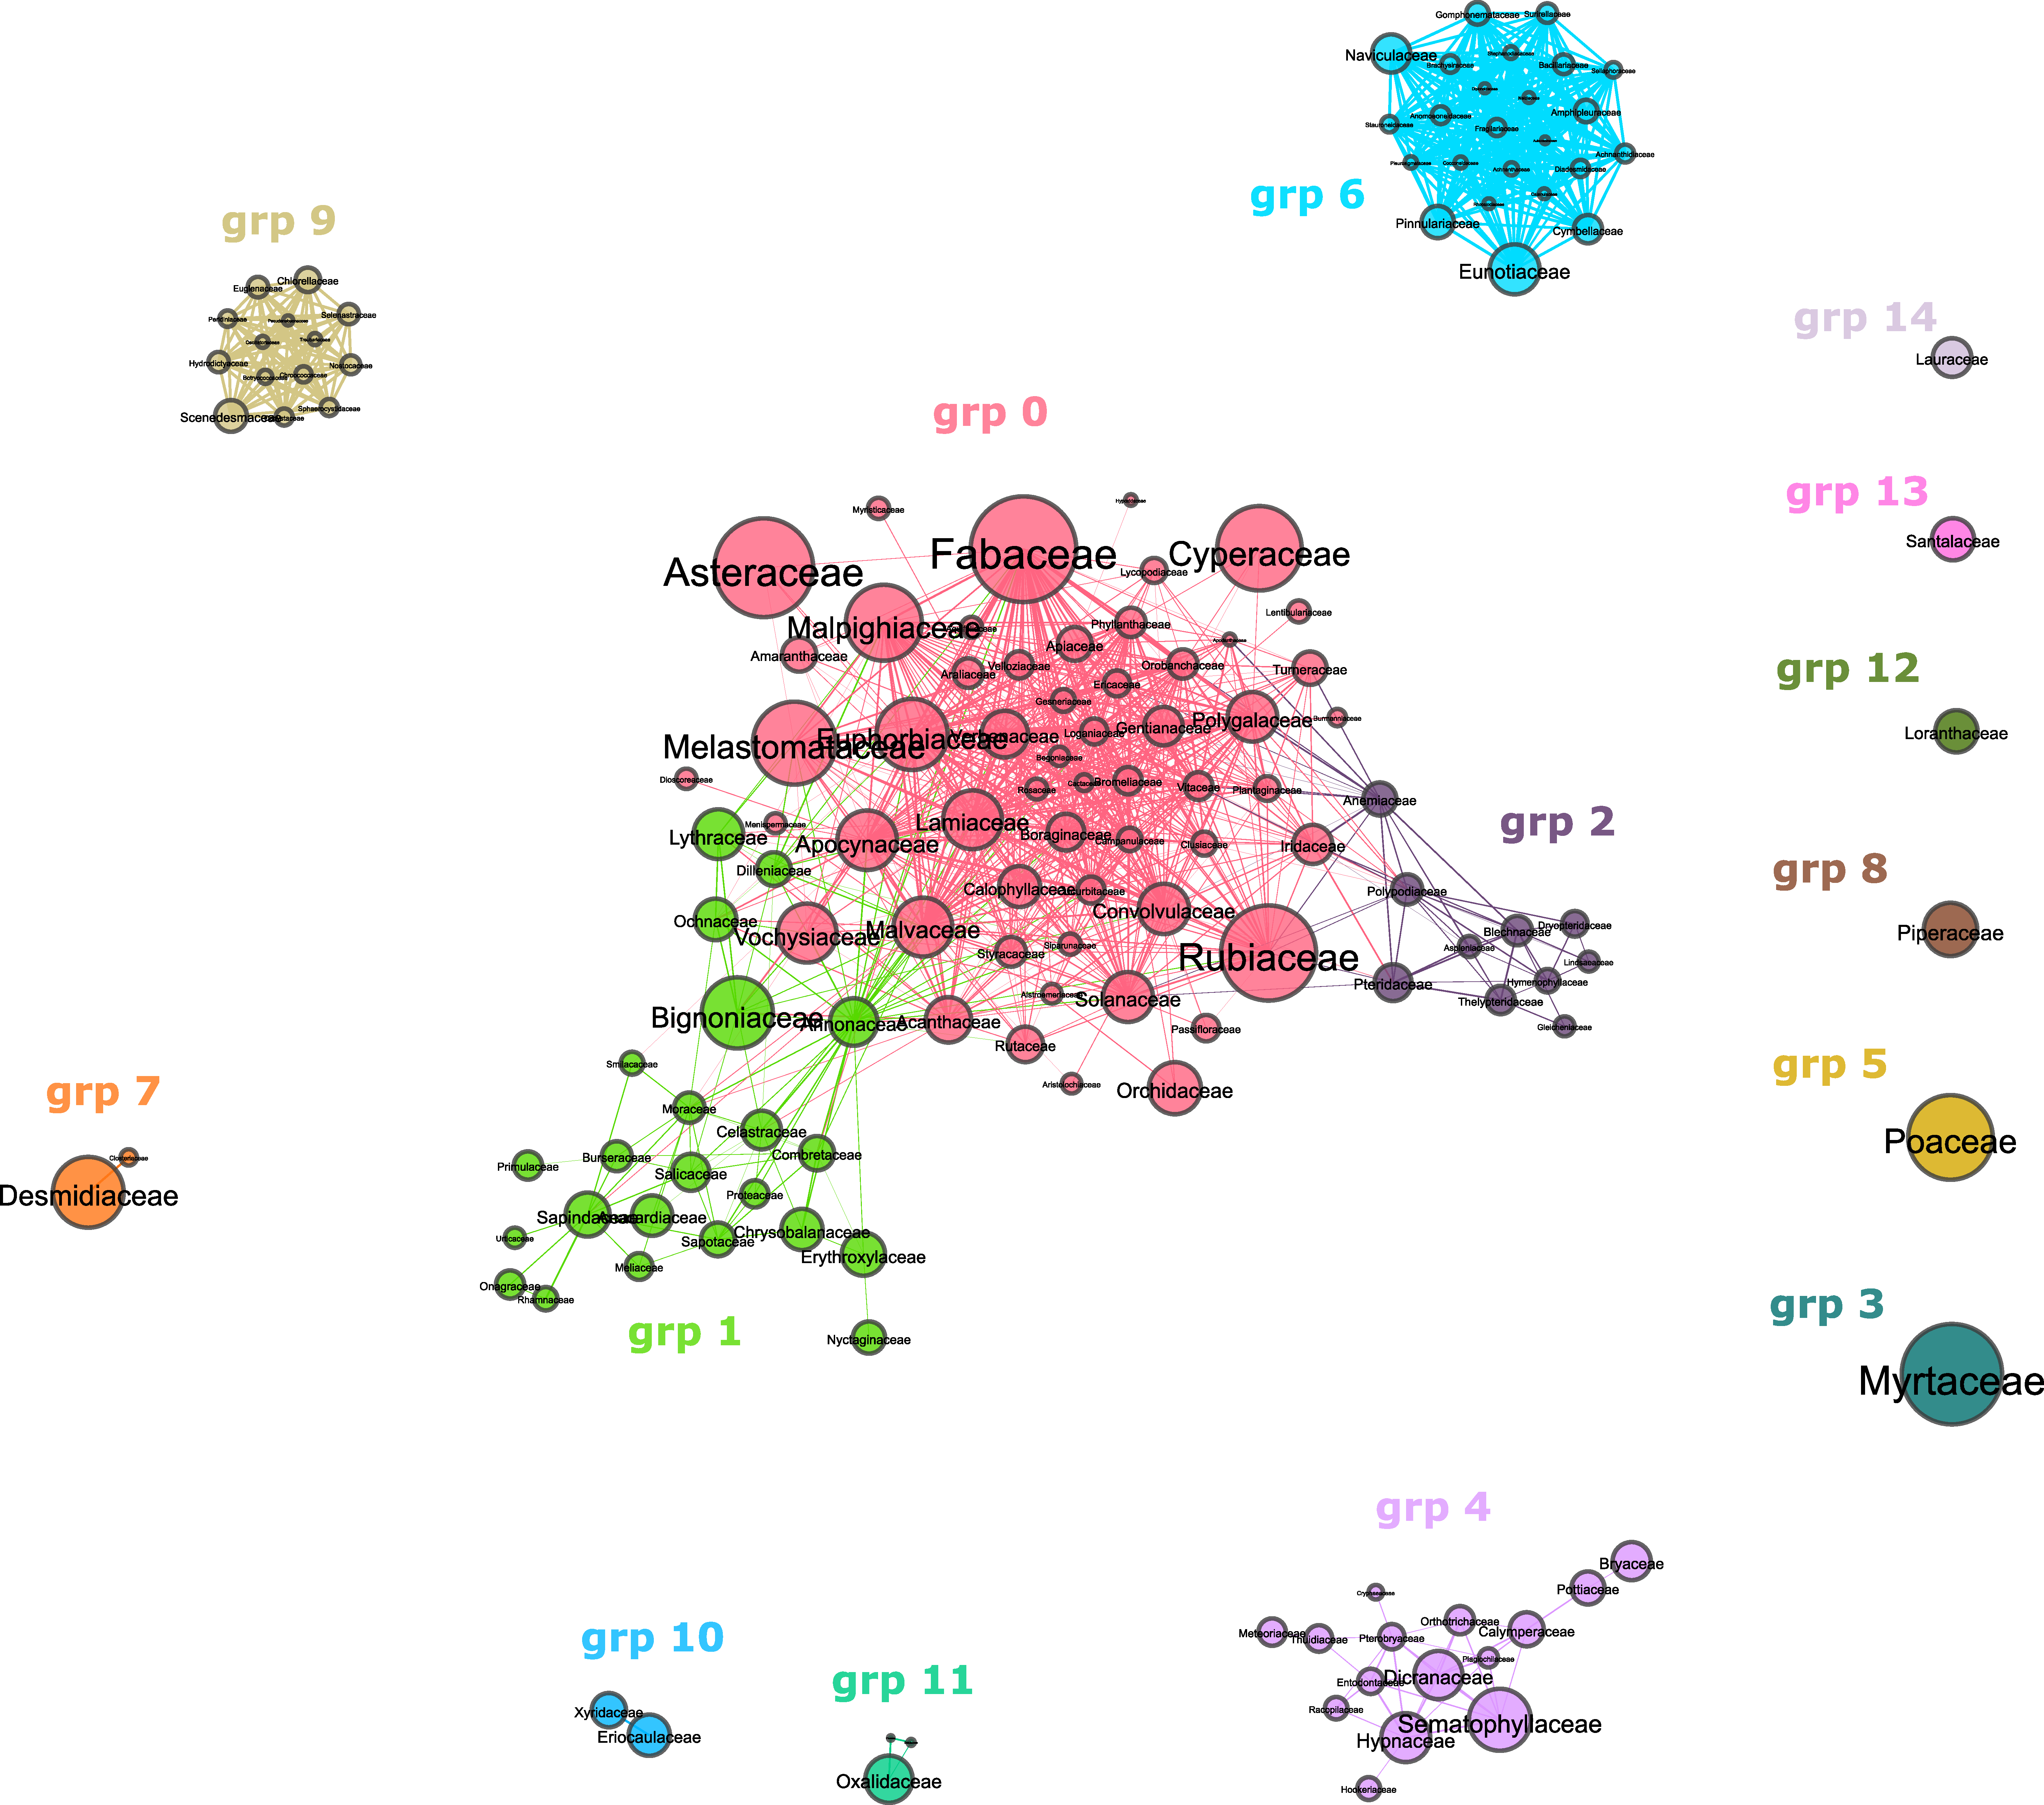
\includegraphics[width=\linewidth]{figures/casestudy_ub/scn_family_projSp_communities.pdf}
    \caption{ Communities in the species projection of the family-aggregated SCN in figure \ref{fig:ub_scn_agg_family_general}, in which edges with weights lower than $20$ were removed as well as isolated nodes. In order to improve visualization, communities with scores lower than $600$ were also omitted from the figure. Colors are used to distinguish communities and nodes sizes reflect families prevalence in the dataset.}
    \label{fig:ub_scn_family_projSp_communities}
\end{figure}

The species projection of the family-aggregated UB SCN network is a one-mode network exclusively representing taxa at the family resolution, with a total of $474$ nodes, $43756$ edges and average node degree of $184$.
Edges between pairs of taxa are weighted according to their quorum vector similarities, such that strongly connected taxa are those which have been recorded by similar sets of collectors, in similar proportions.
%
The relatively low number of nodes observed in the species projection if compared to the collectors projection stands from the fact that in this case the taxonomic aggregation process does reduce the total number of nodes in the network.
While aggregations at higher taxonomic ranks would result in networks with fewer nodes, network density tends to increase as an effect of the summarization of entities and their ties.
%
It is also important to observe that although the absolute number of nodes and edges in the species-projected network are lower than those from the collectors projection, it is still denser than the latter, with a density score of $3.9 \times 10^{-1}$.

% Filtering
In order to reduce network density and better visualize the formation of communities we performing a filtering routine to remove less relevant families associations, analogously to what we've done for the collectors projection.
As network density decreases with increasing values for $\phi$ (Figure \ref{fig:ub_scn_filter_thresh}(b)), we again set the threshold value to $0.8$, omitting ties that are weaker than the threshold value. 
As the process produces many islands, we use the same relevance score from the collectors projection for filtering out non-relevant components, though now using a threshold value of $600$.
The resulting network is shown in Figure \ref{fig:ub_scn_family_projSp_communities}.
Nodes were sized based on the \textit{count} attribute, which indicates how common each family is in the herbarium dataset or, in other words, their \textit{prevalence}. 
Nodes colors reflect the communities they've been assigned to, using the same approach as we did for the collectors projection.

% Communities description
% TODO rephrase
The species projection has a total of $15$ communities, three of which belong to the giant component. 
%
The largest community is \textit{grp $0$}, containing families that are, in general, more widely recorded by herbarium collectors, as it is the case of \textit{Fabaceae}, \textit{Euphorbiaceae} and \textit{Rubiaceae}.
Most of them form a densely-connected structure, containing central families that are all recorded by a very similar set of collectors.
However, there are some families included in the same community which are more loosely connected, and would quickly become isolated nodes if we continued to increase $\phi$. 
This is the case for families \textit{Asteraceae}, \textit{Cyperaceae} and \textit{Orchidaceae}, which indicates that they are recorded by more specialized collectors.
These families are also prevalent in the herbarium dataset.

Community $2$ is composed by fern families (gymnosperms), thus also reflecting a taxonomic group of interest.
Some of the included families are more recorded by fern specialist collectors, as it is the case of \textit{Gleicheniaceae}, \textit{Dryopteridaceae} and \textit{Hymenophyllaceae}.
Others as \textit{Pterydaceae}, \textit{Anemiaceae} and \textit{Polypodiacea} are recorded by collectors who also record flowering plants such as families \textit{Rubiaceae} and \textit{Iridaceae}.


The remaining $12$ communities are all equivalent to islands, $6$ of which formed by isolated nodes.

Community $4$ contains bryophyte families, mostly recorded by collectors within polygon $(i)$ in Figure \ref{fig:ub_scn_agg_family_general}.

Community $6$ contains algae families, mostly diatoms (polygon $(iii)$ in Figure \ref{fig:ub_scn_agg_family_general}).

Communities $9$ and $7$ are composed by green algae families recorded by collectors within polygon $(ii)$ in Figure \ref{fig:ub_scn_agg_family_general}.
As `\textit{leite,alta}' is substantially distinct from `\textit{grando,cw}' and `\textit{castelo-branco,}' regarding their recording interests, families \textit{Desmidiaceae} and \textit{Closteriaceae} are included in a distinct island.

Families \textit{Myrtaceae} (\textit{grp $3$}) and \textit{Poaceae} (\textit{grp $5$}) are both very prevalent in the herbarium and are isolated.
This indicates that they are recorded by more specialized collectors.




% ====================
% Assortativity in SCN
% TODO
% Do collectors who have recorded many taxa (generalists) tend to record taxa recorded by many collectors (generalists)? The inverse also holding.

% Network resilience: If the SCN is dissortative, then it is easier to break it by removing hubs (therefore forming many specialized subgroups of collectors). Otherwise, removing any of the main hubs would not have a considerable effect on fractioning the network (Specialized communities are unlikely to be formed if an important collector leaves the herbarium). 


% Conclusion
Communities discussed above are composed by collectors that share interests in common taxa and, conversely, taxa that has been sampled by a common set of collectors.
These are interest networks.
They do not represent collaborative ties between collectors in field.
This can be investigated with CWN models, as described below.



% ===============================
% UB Collectors Coworking Network
% -------------------------------
% TODO Figure degree dist.
% TODO Figure communities (edges weighted with hyperbolic weighting)


\subsection{The UB Collectors Coworking Network}
% TODO: Add average path size connecting collectors
% From table \ref{table:ub_collectors_florescer}, \textit{Irwin} mostly contributed to the UB herbarium from year $1962$ to $1976$, in the context of the Central Brazil Expedition carried out by the New York Botanical Garden \footnote{\url{http://sciweb.nybg.org/science2/hcol/planalto/index.asp}}. Together with \textit{William R. Anderson} (\textit{anderson,wr}), \textit{Irwin} was a key member of the expedition staff. 

As the UB was built based on the same set of records as the SCN model explored in the previous section, the number of nodes is $6768$, equivalent to the number of collectors nodes in the SCN model.
A total of $10391$ edges represent collaborative ties between collectors.
The average degree and density for the overall network are, respectively, $3.07$ and $4.5 \times 10^{-4}$.

\paragraph*{Connected components.}
The UB CWN network is composed by a a total of $2991$ connected components, from which the largest one --- the giant component ($c_1$) ---  contains $46\%$ of all nodes in the network.
Such a low percentage of nodes in the giant component contrasts to most empirical scientific paper-publishing collaboration networks studied by Newman in one of his $2001$ papers \cite{Newman2001d}, for which the giant components contain as much as $80\% - 90\%$ of all nodes.
Moreover, only $318$ of the connected components ($c_1, c_2, ..., c_{318}$) are composed by collectors with at least one collaborative tie.
The remaining $2673$ components ($c_{319}, c_{320}, ..., c_{2991}$) are all disconnected nodes (\textit{i.e.} nodes with $k=0$), which we refer to as \textit{singleton} collectors.

Singleton collectors are those who have never recorded specimens collaboratively --- or at least they have not included the names of their collaborators in the records as authors ---, and thus are considered to have no structural role in the collaboration network.
They comprise $39.5\%$ of all nodes in the network, and the fact that they lack connections impacts on the overall network density, making it relatively low.
In fact, if we instead compute network density by only considering nodes from the giant component $c_1$, we observe an increase from $4.5 \times 10^{-4}$ to $1.95 \times 10^{-3}$. 

One important example of a singleton collector is `\textit{leite,alta}', with a total of $2757$ records, none of which collaborative (inset in Figure~\ref{fig:ub_team_sizes}).  % of records from all singleton collectors
This comprises $18.14\%$ of all records by singleton collectors.
All other $2672$ singleton collectors have fewer than $400$ records each.
Moreover, $81.1\%$ of occurrences recorded by a singleton collector have been obtained in Brazil.

% Low-degree isolated nodes are probably experienced foreign collectors (who have only contributed to the herbarium with few records (probably exchanges)), as it is unlikely that novice collectors would record alone, without a supervisor. -> Apparently not true


\paragraph*{How collaborative are collectors?}
% We use metrics such as average degree, degree distribution, ... as measures of collector collaborativity.

% Team sizes
By inspecting team sizes of all records in the dataset, we find that the average team size for records in the UB dataset is $1.73$, as a consequence of the fact that $63\%$ of all records are non-collaborative, \textit{i.e.} recorded by a single collector (Figure \ref{fig:ub_team_sizes}).
%
Records distribution seems to decay logarithmically with team size, at least for teams with sizes varying from $1$ to $8$.
For some reason which is not clear for us, records above $8$ are apparently forbidden in the dataset (we consider the single record with team size $9$ to be an artifact).
One hypothesis to be verified is that some mechanism specific to the data management system used by UB constrains the maximum number of collectors allowed for each record.
In some records the string containing the collectors names are truncated, which also could also indicate a system-specific constrain towards the maximum string length.

\begin{figure}[!h]
  	\centering
    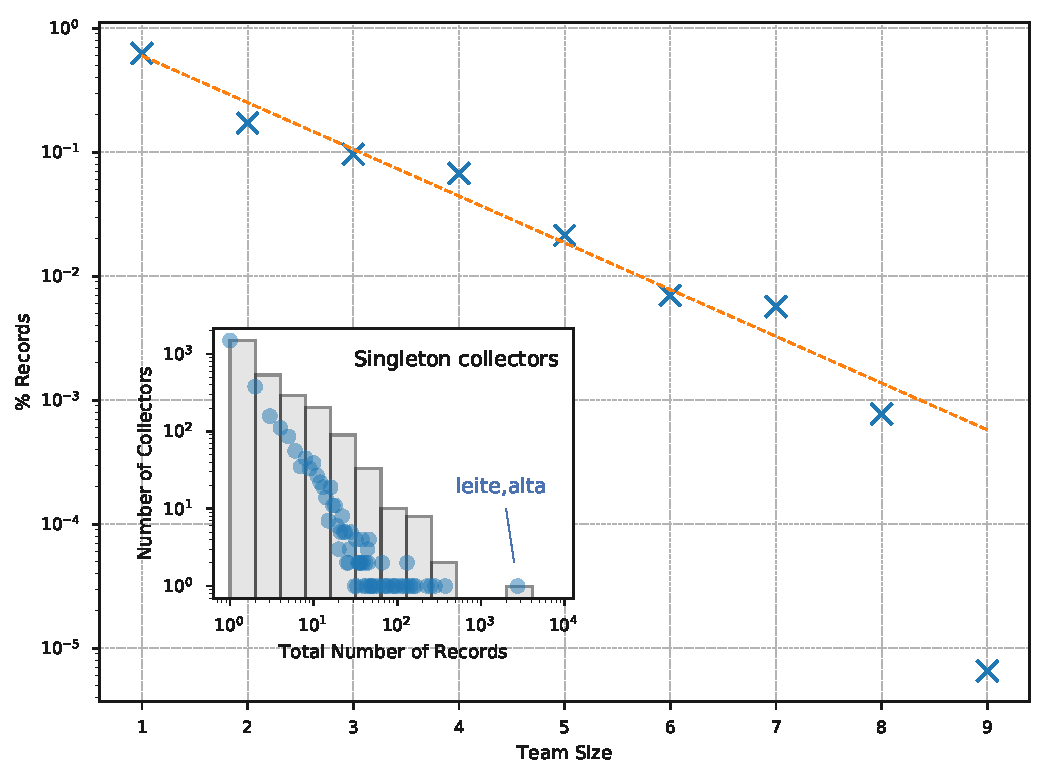
\includegraphics[width=0.9\linewidth]{figures/casestudy_ub/team_sizes.pdf}
    \caption{ Percentage of occurrence records in the UB dataset for each team size. The orange line represents an exponential fit to the data (using team sizes from $1$ to $8$) using function $f(x) = 10^{\beta_0 + \beta_1 x}$ and parameters $\beta_0=0.16$ and $\beta_1=-0.38$. The inset figure shows the number of records singleton collectors typically hold, with records numbers logarithmically binned using base $2$. }
    \label{fig:ub_team_sizes}
\end{figure}

Collectors in the UB CWN vary substantially regarding their collaborativeness during fieldwork.
Whereas few ones have collaborated with a large number of collectors throughout their careers (much more than the average $3.07$), almost $40\%$ of them have never co-authored a single record.
The existence of so many singleton collectors in the dataset (with $k=0$ explains the relatively low average degree score if we consider the entire network. 

If we consider the entire CWN network, collectors collaborate, in average, with $3.07$ distinct collectors throughout their entire careers, which is lowered by the existence of many singleton collectors in the dataset, with $k=0$.
If we only consider the giant component, $\langle k\rangle = 6.08$.
If we exclude the giant component, $\langle k\rangle = 0.51$. 
The average degree lower than $1$ is explained by the existence of so many singleton collectors.

Similarly to the SCN network, degree distribution for the CWN network does not fit a poisson distribution well (which is characteristic of random networks). 
It fits better a power law with parameter $\alpha=2.2$.

%% degree dist. FIGURE %%
\begin{figure}[!ht]
  	\centering
    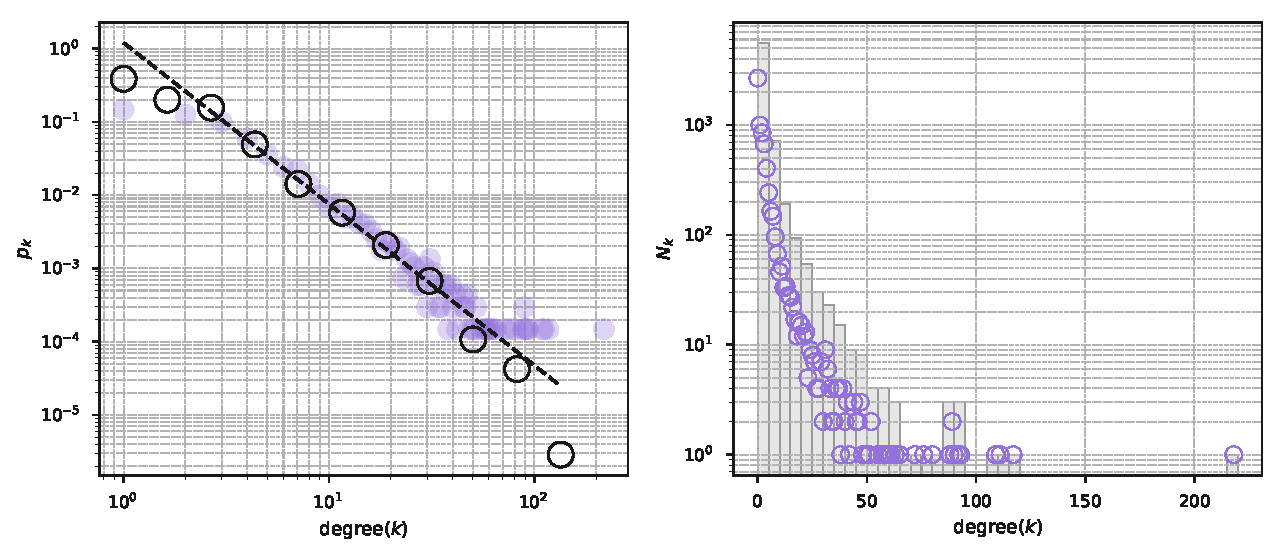
\includegraphics[width=\linewidth]{figures/casestudy_ub/cwn_degree_dist.pdf}
    \caption{ Degree Dist.}
    \label{fig:ub_cwn_degree_dist}
\end{figure}

Depending on the degree centrality metric we use, we get a different ranking of most influential collectors.
The non-weighted degree $k$ ranks collectors based on the total number of collaborations they've established to distinct collectors, irrespective of the number of times each association was observed.
We might want to consider the number of recurrent collaborations with each collaborator, by using the weighted degree metric.
If we use the weighted degree $k_w$ metric, we must specify which weighting rule to use. 
If we use the edge \textit{count} attribute, which is simply the number of times a given association between two collectors occur, the weighted degree for each collector is equivalent to his/her total number of collaborative records. 

We could use another weighting rule for calculating the $k_w$ centrality, for example the hyperbolic weighting.

\begin{table}[H]
  \caption{}
  \begin{center}
  \begin{tabular}{l r r r r}
      collector & num of records & \% collaborative & $k$ & $k_w$ \\
      \hline
      irwin,hs & 18065 & 34.1 & 39 & 5696.0 \\
      proenca,ceb & 4803 & 88.3 & 218 & 4203.7 \\
      faria,jeq & 4687 & 82.9 & 117 & 3881.0 \\
      souza,rr & 3885 & 99.3 & 37 & 3835.5 \\
      santos,rrb & 3587 & 94.5 & 41 & 3382.3 \\
      munhoz,cbr & 3191 & 82.8 & 109 & 2493.2 \\
      zanatta,mrv & 2364 & 95.8 & 50 & 2264.0 \\
      castelobranco,cw & 2256 & 100.0 & 1 & 2256.0 \\
      grando,jv & 2256 & 100.0 & 1 & 2256.0 \\
      eiten,g & 3046 & 61.4 & 33 & 1865.5 \\
      amaral,ag & 1825 & 99.5 & 37 & 1815.0 \\
      projetobiodiversidadebp & 1780 & 100.0 & 19 & 1780.0 \\
      mendes,vc & 1696 & 99.9 & 89 & 1695.0 \\
      fonseca,sf & 1610 & 99.9 & 18 & 1607.0 \\
      camara,peas & 2076 & 79.8 & 47 & 1486.0 \\
      harley,rm & 2564 & 66.0 & 90 & 1455.8 \\
      carvalhosilva,m & 1635 & 98.5 & 58 & 1436.0 \\
      eiten,lt & 1262 & 99.6 & 14 & 1256.5 \\
      mello,trb & 1247 & 100.0 & 21 & 1247.0 \\
      soares,aer & 1557 & 73.0 & 29 & 1135.0 \\
      \hline
  \end{tabular}
  \label{table:ub_cwn_}
  \end{center}
\end{table}
%% FIGURE HERE %%

% TODO: WRONG!! Remember that k_w using count attribute does not give the absolute number of collaborative records!
For a concrete example, \textit{Howard S. Irwin} (\textit{irwin,hs}) is the top collector in terms of absolute number of collaborative ties. He has collected a total of $14803$ specimens in field with others. However, the network indicates that he usually works with a more restricted team of partners. He holds only $39$ links to distinct collectors, which puts him in the $43th$ position of the rank. 
On the other hand, \textit{James A. Ratter} (\textit{ratter,ja}), who is the third with most connections to distinct collectors, is at the $20th$ position in the $k_w$ rank, with a total of $2962$ collaborative collectors.
There are only $3$ collectors in common between the top-10 collectors in the $k_w$ and the $k$ ranks.
% TODO: Include hyperbolic weighting (and compare with degree k)

\paragraph*{Coworking groups.}
\begin{figure}[!ht]
  	\centering
    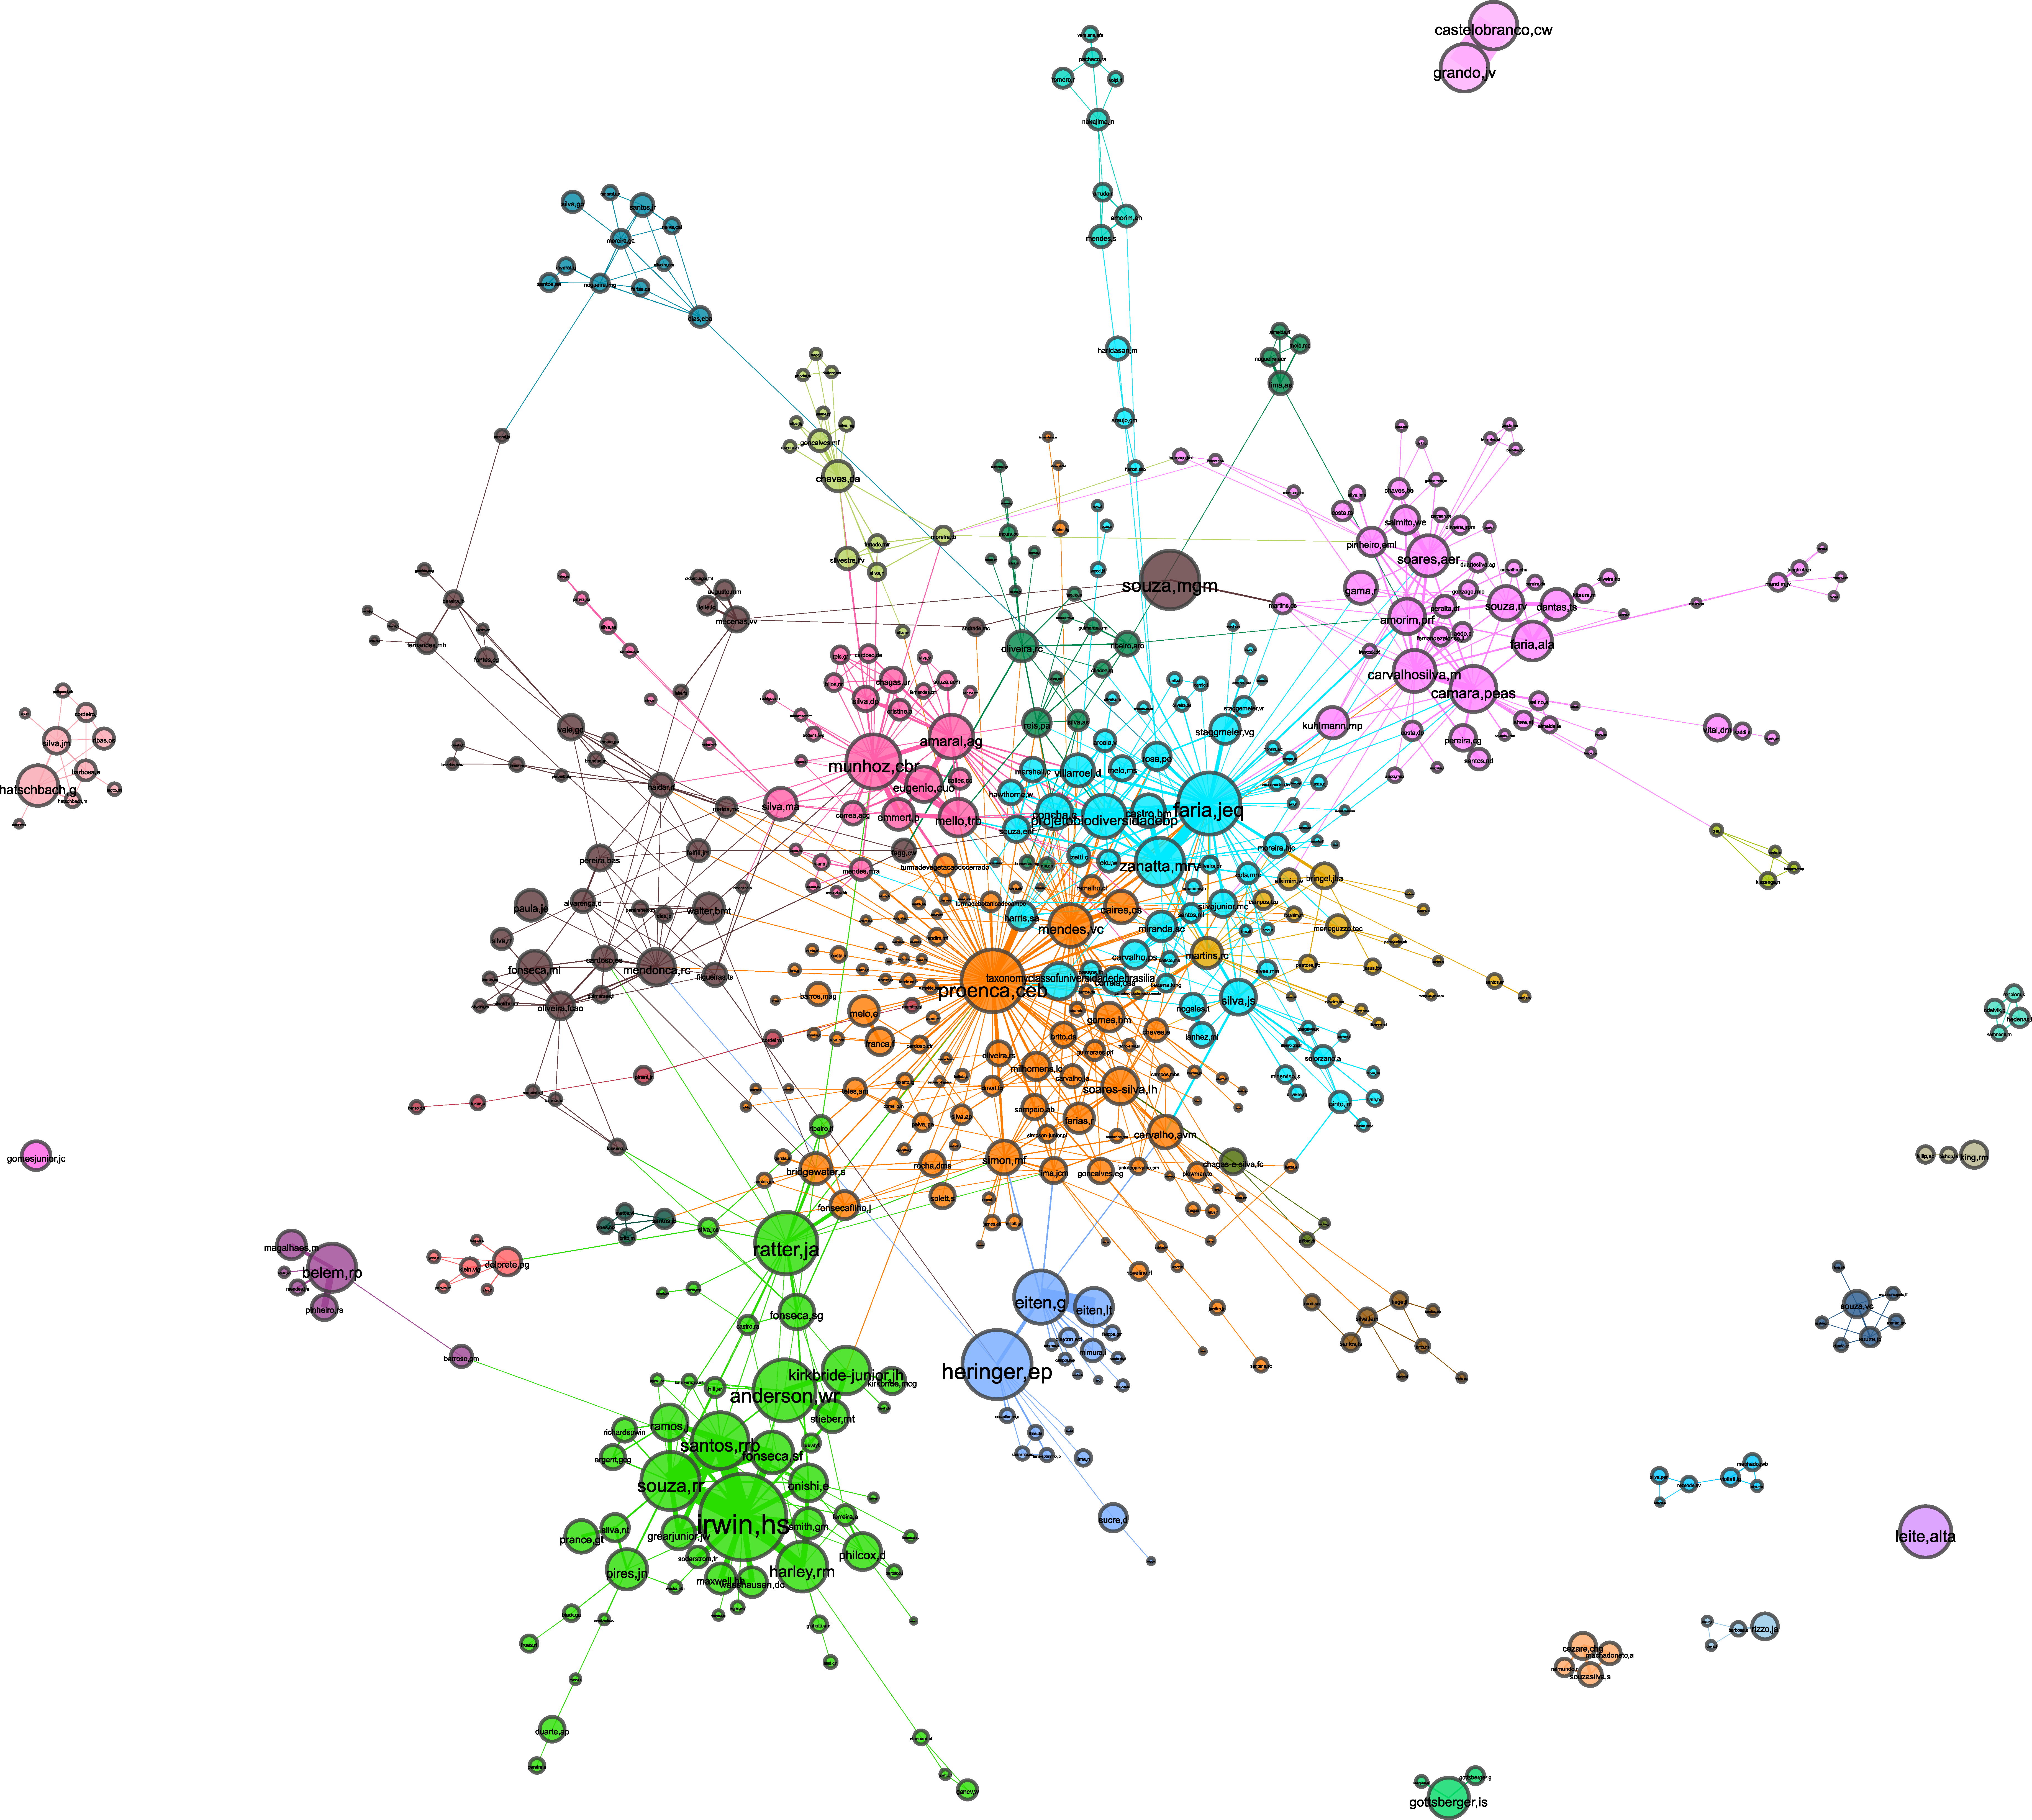
\includegraphics[width=\linewidth]{figures/casestudy_ub/cwn_communities.pdf}
    \caption{ Coworking groups.}
    \label{fig:ub_cwn_communities}
\end{figure}

% Assortativity
\paragraph*{Do collaborative collectors prefer to work with others who are also collaborative?}
One relevant question we might ask is whether collectors tend to form collaborative ties preferentially with others holding a similar number of collaborative ties.
Here we refer to collaborative collectors as those holding collaborative ties with many distinct collectors, irrespective of the number of times each individual link occurs. Those collectors which hold strong collaborative ties with few collaborators are thus less collaborative than the former case. In this sense, $proenca,ceb$ is considered more collaborative than $irwin,hs$, for instance.

More concretely, we want to assess whether the network is assortatively mixed.
If this is the case then we would expect to observe that most collaborators of very collaborative collectors are also very collaborative.
Conversely, collectors that do not hold many ties, for instance novice or non-collaborative experienced collectors, should preferentially connect with others with similar degrees.
This would lead to a network where highly collaborative collectors are clustered together, composing a solid core. Less collaborative ones would, instead, tend to be marginalized. % TODO: add a figure comparing those patterns

For assessing network mixing pattern we calculated the Pearson correlation coefficient $r = \frac{\sum_{xy} xy(e_{xy}-a_xb_y)}{\sigma_a \sigma_b}$ , as proposed by Newman \cite{Newman2003c} (eq. 21).
The term $e_{xy}$ represents the fraction of edges that connect nodes with degrees $x$ and $y$ in the network, such that $\sigma_{xy}e_{xy}=1$. 
Computing the correlation coefficient involves comparing the term $e_{xy}$ with the product between the percentage of all edges that start in a $x$-degree node ($a_x$) and the percentage of all edges that end in a $y$-degree node ($b_y$). The computation is carried out for each combination of degree values $x$ and $y$.
By using this metric we assess whether a correlation exists between the degrees of each pair of nodes which are connected by an edge. 
The result is bound to the $[-1,1]$ interval, where a score of $1$ indicates perfect assortativity and a score of $-1$, perfect dissortativity.
Scores close to $0$ indicate that no correlation exists between nodes, and thus the network is neither assortative nor dissortative.

For the UB collectors coworking network we obtained an assortativity score of $-0.0034$ for the network as a whole, including all the isolated components; and a score of $-0.0308$ only considering the giant component.
Both coefficients are negative and very close to zero, suggesting that collectors do collaborate with others irrespectively of their degrees. In other words, we do not observe a significant degree correlation between nodes in this network. 
This result contrasts with those from Newman's paper \cite{Newman2003b}, which shows that typically social networks display assortative mixing. Additionally states that this is one of the aspects that differentiate social networks differentiate from other types of networks. In other words, high degree nodes tend to associate to other high-degree ones. Nodes tend to associate to others of similar degree.
This is not the case for the CWN network. If we consider the network as whole, including the many isolated components, we get an assortativity coefficient of $-0.0034$, whereas if we consider only the giant component it is $-0.0308$. 
% but check {Bearman2004}... similar assortativity


% TODO: Betweeness: Which collectors facilitate collaborative behavior?
 
 



%%% QUESTIONS

%% 1. How common are collaborative recordings within the dataset?
%%% What is the proportion of collaborative records in the dataset? How many collaborators
%%% One-collector recording vs >2 collectors recordings
%%% Distribution of team size
%%% Caveats: Some collectors may not include collaborators names in the records

%% x. How likely is a novice collector to become a great collector?

%% x. Do collectors with similar interests tend to collect together?
%%% Mix of the two models
%%% Look for homophily in collectors communities, assortativity.

%% x. Which groups of species best partitionate collectors in the dataset, in terms of their collection interests? 
%%% Using SCNs
%%% Are these groups necessarily taxonomic ones (such as family)? Or could functional groups be more relevant in some cases? Or is there a geographical effect?
%%% e.g. Some group might be best classified as specialists on species inhabiting some geographical location, with some specific habit and belonging to some family rather than simply as specialists in a given family.

%% x. The Expert-location problem {Chapt. 8 of book Social Network Data Analytics}
%%% The expert team formation problem: How can we best select experts for a given job, based on how willing they are of collaborating together?
%%% Combine both SCN and CWN
\newcounter{QuestionsCounter}
\setcounter{QuestionsCounter}{1}

\subsubsection*{Question \arabic{QuestionsCounter}: What team sizes do collectors usually form?}
% Average team sizes

\stepcounter{QuestionsCounter}
\subsubsection*{Question \arabic{QuestionsCounter}: <Another question>}

\stepcounter{QuestionsCounter}
\subsubsection*{Question \arabic{QuestionsCounter}: Who are specialist/generalist collectors?}
% References {Newman2004}


% Statistical characterization of CWN structure
%% Largest component, connected components...
%% Assortativity: Do collectors with many collaborators (very collaborative) tend to associate with others that are also very collaborative?






%\subsection{Features Selection}

%% Features engineering

%\section{Model Evaluation}

